% ------------------------------------------------------------------------
% ------------------------------------------------------------------------
% Modelo UFSC para Trabalhos Academicos (tese de doutorado, dissertação de
% mestrado) utilizando a classe abntex2
%
% Autor: Alisson Lopes Furlani
% 	Modificações:
%	- 27/08/2019: Alisson L. Furlani, add pacote 'glossaries' para listas
%   - 06/11/2019: Luiz-Rafael Santos, modifica para Trabalho de Conclusão de Curso
% ------------------------------------------------------------------------
% ------------------------------------------------------------------------

\documentclass[
	% -- opções da classe memoir --
	12pt,				% tamanho da fonte
	%openright,			% capítulos começam em pág ímpar (insere página vazia caso preciso)
	oneside,			% para impressão no anverso. Oposto a twoside
	a4paper,			% tamanho do papel. 
	% -- opções da classe abntex2 --
	chapter=TITLE,		% títulos de capítulos convertidos em letras maiúsculas
	section=TITLE,		% títulos de seções convertidos em letras maiúsculas
	%subsection=TITLE,	% títulos de subseções convertidos em letras maiúsculas
	%subsubsection=TITLE,% títulos de subsubseções convertidos em letras maiúsculas
	% -- opções do pacote babel --
	english,			% idioma adicional para hifenização
	%french,				% idioma adicional para hifenização
	%spanish,			% idioma adicional para hifenização
	brazil				% o último idioma é o principal do documento
	]{abntex2}

\usepackage{setup/ufscthesisA4-alf}

% ---
% Filtering and Mapping Bibliographies
% ---
% Pacotes de citações
% ---
\usepackage{csquotes}
\usepackage[backend = biber, style = abnt]{biblatex}
% FIXME Se desejar estilo numérico de citações,  comente a linha acima e descomente a linha a seguir.
% \usepackage[backend = biber, style = numeric-comp]{biblatex}

\setlength\bibitemsep{\baselineskip}
\DeclareFieldFormat{url}{Disponível~em:\addspace\url{#1}}
\NewBibliographyString{sineloco}
\NewBibliographyString{sinenomine}
\DefineBibliographyStrings{brazil}{%
	sineloco     = {\mkbibemph{S\adddot l\adddot}},
	sinenomine   = {\mkbibemph{s\adddot n\adddot}},
	andothers    = {\mkbibemph{et\addabbrvspace al\adddot}},
	in			 = {\mkbibemph{In:}}
}

\addbibresource{aftertext/references.bib} % Seus arquivos de referências

% ---
\DeclareSourcemap{
	\maps[datatype=bibtex]{
		% remove fields that are always useless
		\map{
			\step[fieldset=abstract, null]
			\step[fieldset=pagetotal, null]
		}
		% remove URLs for types that are primarily printed
%		\map{
%			\pernottype{software}
%			\pernottype{online}
%			\pernottype{report}
%			\pernottype{techreport}
%			\pernottype{standard}
%			\pernottype{manual}
%			\pernottype{misc}
%			\step[fieldset=url, null]
%			\step[fieldset=urldate, null]
%		}
		\map{
			\pertype{inproceedings}
			% remove mostly redundant conference information
			\step[fieldset=venue, null]
			\step[fieldset=eventdate, null]
			\step[fieldset=eventtitle, null]
			% do not show ISBN for proceedings
			\step[fieldset=isbn, null]
			% Citavi bug
			\step[fieldset=volume, null]
		}
	}
}
% ---

% ---
% Informações de dados para CAPA e FOLHA DE ROSTO
% ---
% FIXME Substituir 'Nome completo do autor' pelo seu nome.
\autor{Matheus Souza Rozendo}
% FIXME Substituir 'Título do trabalho' pelo título da trabalho.
\titulo{Bancada de visão computacional de baixo custo para classificação de tomates-cereja}
% FIXME Substituir 'Subtítulo (se houver)' pelo subtítulo da trabalho.  
% Caso não tenha substítulo, comente a linha a seguir.
\subtitulo{maturação por tabela de consulta de cores e defeitos por rede neural convolucional}
% FIXME Substituir 'XXXXXX' pelo nome do seu
% orientador.
\orientador{Prof. XXXXXX, Dr.}
% FIXME Se for orientado por uma mulher, comente a linha acima e descomente a linha a seguir.
% \orientador[Orientadora]{Nome da orientadora, Dra.}
% FIXME Substituir 'XXXXXX' pelo nome do seu
% coorientador. Caso não tenha coorientador, comente a linha a seguir.
\coorientador{Prof. XXXXXX, Dr.}
% FIXME Se for coorientado por uma mulher, comente a linha acima e descomente a linha a seguir.
% \coorientador[Coorientadora]{XXXXXX, Dra.}
% FIXME Substituir 'XXXXXX' pelo nome do Coordenador do 
% programa/curso.
\coordenador{Prof. XXXXXX, Dr.}
% FIXME Se for coordenadora mulher, comente a linha acima e descomente a linha a seguir.
% \coordenador[Coordenadora]{Nome da Coordenadora, Dra.}
% FIXME Substituir '[ano da entrega]' pelo ano (ano) em que seu trabalho foi defendido.
\ano{2026}
% FIXME Substituir '[dia] de [mês] de [ano]' pela data em que ocorreu sua defesa.
\data{[dia] de [mês] de [ano]}
% FIXME Substituir '[Cidade da defesa]' pela cidade em que ocorreu sua defesa.
\local{[Cidade da defesa]}
\instituicaosigla{UFSC}
\instituicao{Universidade Federal de Santa Catarina}
% FIXME Substituir 'Dissertação/Tese' pelo tipo de trabalho (Tese, Dissertação). 
\tipotrabalho{Trabalho de Conclusão de Curso}
% FIXME Substituir '[licenciado/bacharel] em [nome do título obtido]' pela grau adequado.
\formacao{[licenciado/bacharel] em [nome do título obtido]}
% FIXME Substituir '[licenciado/bacharel]' pelo nivel adequado.
\nivel{[licenciado/bacharel]}
% FIXME Substituir 'Curso de Graduação em [XXXXXXXX]' pela curso adequado.
\programa{Curso de Graduação em [XXXXXXXX]}
% FIXME Substituir 'Campus XXXXXX ou Centro de XXXXXX' pelo campus ou centro adequado.
\centro{Campus [XXXXXX] ou Centro de [XXXXXX]}
\preambulo
{%
\imprimirtipotrabalho~do~\imprimirprograma~do~\imprimircentro~da~\imprimirinstituicao~para~a~obtenção~do~título~de~\imprimirformacao.
}
% ---

% ---
% Configurações de aparência do PDF final
% ---
% alterando o aspecto da cor azul
\definecolor{blue}{RGB}{41,5,195}
% informações do PDF
\makeatletter
\hypersetup{
     	%pagebackref=true,
		pdftitle={\@title}, 
		pdfauthor={\@author},
    	pdfsubject={\imprimirpreambulo},
	    pdfcreator={LaTeX with abnTeX2},
		pdfkeywords={ufsc, latex, abntex2}, 
		colorlinks=true,       		% false: boxed links; true: colored links
    	linkcolor=black,%blue,          	% color of internal links
    	citecolor=black,%blue,        		% color of links to bibliography
    	filecolor=black,%magenta,      		% color of file links
		urlcolor=black,%blue,
		bookmarksdepth=4
}
\makeatother
% ---

% ---
% compila a lista de abreviaturas e siglas e a lista de símbolos
% ---

% Declaração das siglas
\siglalista{CEAGESP}{Companhia de Entrepostos e Armazéns Gerais de São Paulo}
\siglalista{CEASA}{Central de Abastecimento}
\siglalista{CIE}{Comissão Internacional de Iluminação}
\siglalista{CNN}{Rede Neural Convolucional (\textit{Convolutional Neural Network})}
\siglalista{CSV}{Valores Separados por Vírgula (\textit{Comma-Separated Values})}
\siglalista{FAO}{Organização das Nações Unidas para a Alimentação e a Agricultura}
\siglalista{HSV}{Matiz, Saturação e Valor (\textit{Hue, Saturation, Value})}
\siglalista{IC}{Intervalo de Confiança}
\siglalista{IHM}{Interface Homem-Máquina}
\siglalista{LUT}{Tabela de Consulta (\textit{Look-Up Table})}
\siglalista{MLP}{Perceptron Multicamadas (\textit{Multilayer Perceptron})}
\siglalista{ONNX}{\textit{Open Neural Network Exchange}}
\siglalista{PBMH}{Programa Brasileiro para a Modernização da Horticultura}
\siglalista{ResNet}{Rede Residual (\textit{Residual Network})}
\siglalista{RGB}{Vermelho, Verde e Azul (\textit{Red, Green, Blue})}
\siglalista{RMSE}{Raiz do Erro Quadrático Médio (\textit{Root Mean Square Error})}
\siglalista{USDA}{Departamento de Agricultura dos Estados Unidos (\textit{United States Department of Agriculture})}
\siglalista{YOLO}{\textit{You Only Look Once}}
\simbololista{A}{\ensuremath{A}}{Área do contorno do fruto, em pixels ou mm$^2$}
\simbololista{P}{\ensuremath{P}}{Perímetro do contorno do fruto, em pixels}
\simbololista{k}{\ensuremath{k}}{Número de grupos do \textit{k-means} ou de partes da validação cruzada}

% compila a lista de abreviaturas e siglas e a lista de símbolos
\makenoidxglossaries 

% ---

% ---
% compila o indice
% ---
\makeindex
% ---

% ----
% Início do documento
% ----
\begin{document}

% Seleciona o idioma do documento (conforme pacotes do babel)
%\selectlanguage{english}
\selectlanguage{brazil}

% Retira espaço extra obsoleto entre as frases.
\frenchspacing 

% Espaçamento 1.5 entre linhas
\OnehalfSpacing

% Corrige justificação
%\sloppy

% ----------------------------------------------------------
% ELEMENTOS PRÉ-TEXTUAIS
% ----------------------------------------------------------
% \pretextual %a macro \pretextual é acionado automaticamente no início de \begin{document}
% ---
% Capa, folha de rosto, ficha bibliografica, errata, folha de apróvação
% Dedicatória, agradecimentos, epígrafe, resumos, listas
% ---
% ---
% Capa
% ---
\imprimircapa
% ---

% ---
% Folha de rosto
% (o * indica que haverá a ficha bibliográfica)
% ---
\imprimirfolhaderosto*
% ---

% ---
% Inserir a ficha bibliografica
% ---
% http://ficha.bu.ufsc.br/
%\begin{fichacatalografica}
%	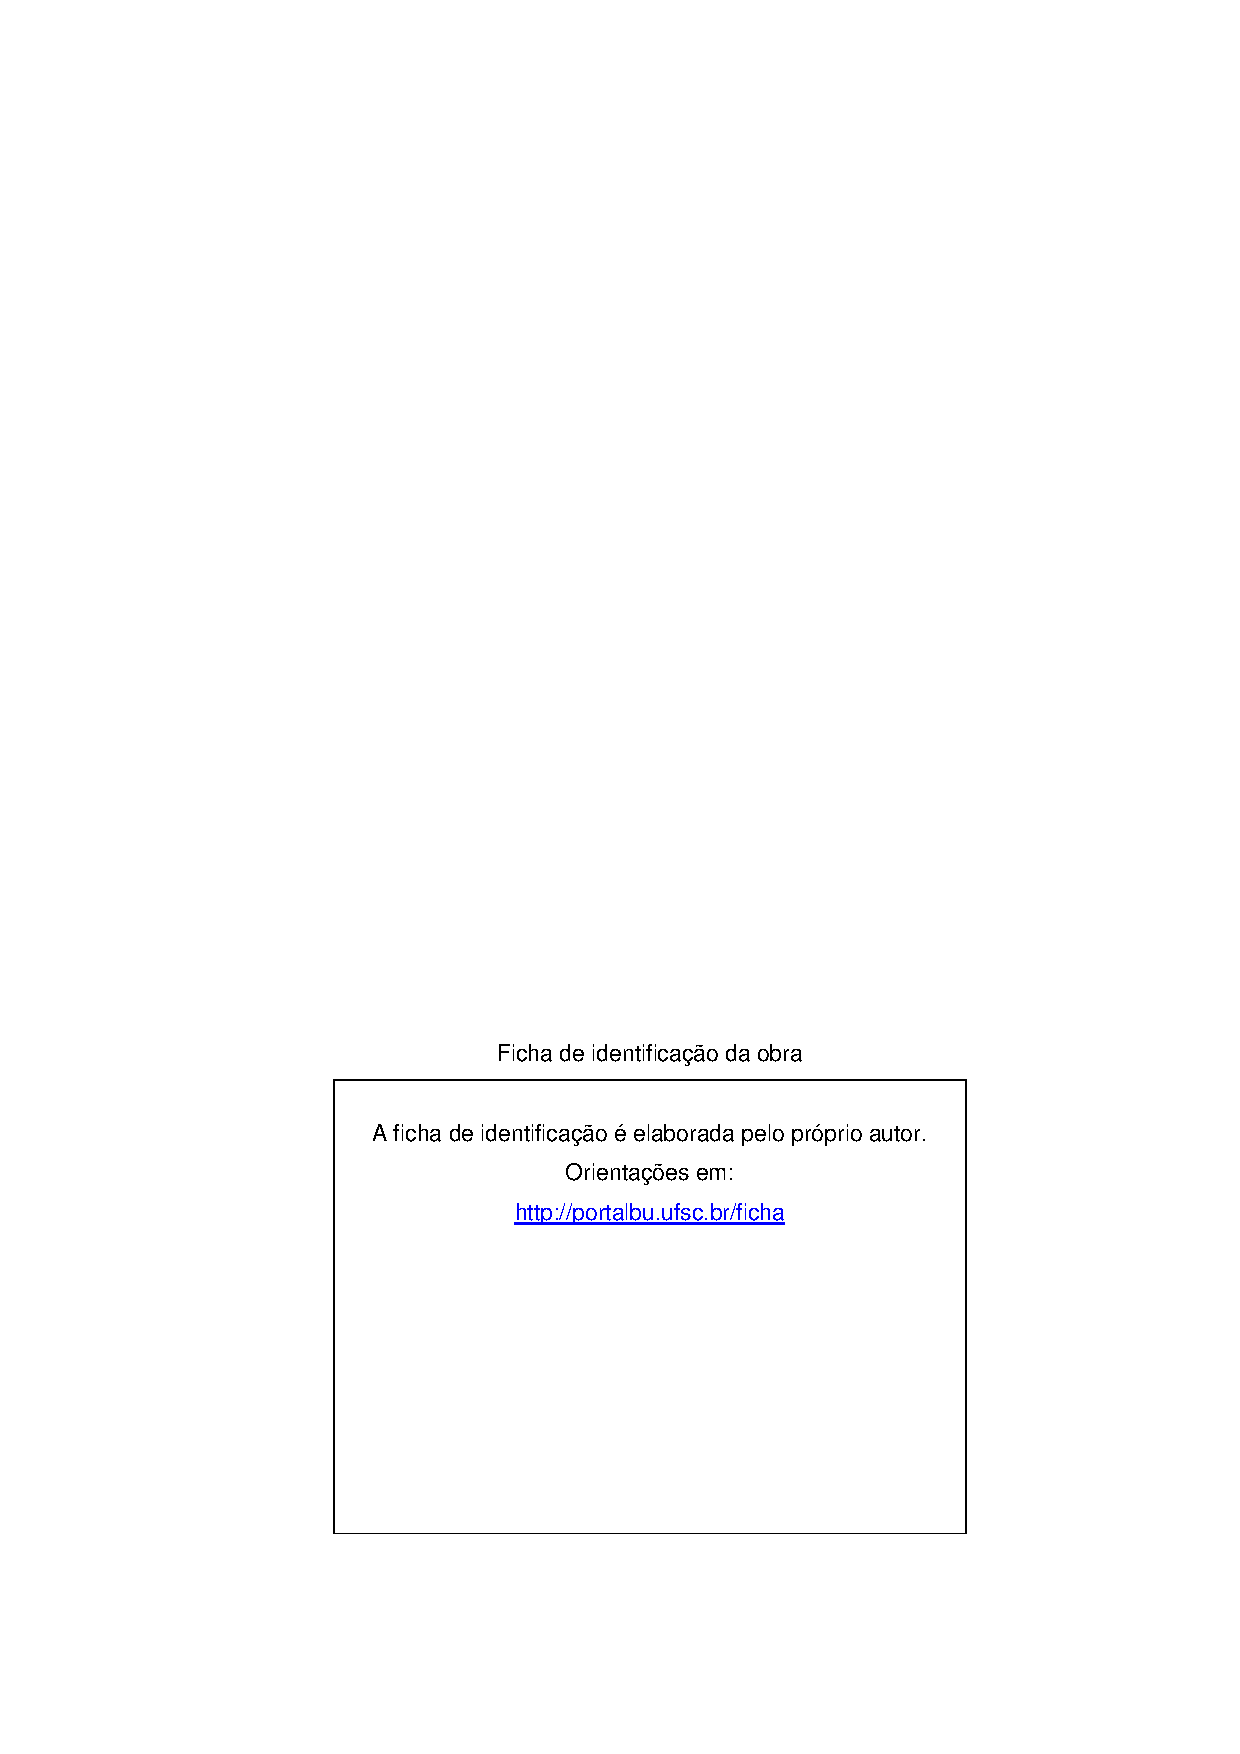
\includepdf{beforetext/Ficha_Catalografica.pdf}
%\end{fichacatalografica}
% ---

% ---
% Inserir folha de aprovação
% ---
%\begin{folhadeaprovacao}
%	\OnehalfSpacing
%	\centering
%	\imprimirautor\\%
%	\vspace*{10pt}		
%	\textbf{\imprimirtitulo}%
%	\ifnotempty{\imprimirsubtitulo}{:~\imprimirsubtitulo}\\%
	%		\vspace*{31.5pt}%3\baselineskip
%	\vspace*{\baselineskip}
	%\begin{minipage}{\textwidth}
	% ~do~\imprimirprograma~do~\imprimircentro~da~\imprimirinstituicao~para~a~obtenção~do~título~de~\imprimirformacao.
%	Este~\imprimirtipotrabalho~foi julgado adequado para obtenção do Título de “\imprimirformacao” e aprovado em sua forma final pelo~\imprimirprograma. \\
%		\vspace*{\baselineskip}
%	\imprimirlocal, \imprimirdata. \\
%	\vspace*{2\baselineskip}
%	\assinatura{\OnehalfSpacing\imprimircoordenador \\ \imprimircoordenadorRotulo~do Curso}
%	\vspace*{2\baselineskip}
%	\textbf{Banca Examinadora:} \\
%	\vspace*{\baselineskip}
%	\assinatura{\OnehalfSpacing\imprimirorientador \\ \imprimirorientadorRotulo}
	%\end{minipage}%
%	\vspace*{\baselineskip}
%	\assinatura{Prof.(a) xxxx, Dr(a).\\
%	Avaliador(a) \\
%	Instituição xxxx}

%	\vspace*{\baselineskip}
%	\assinatura{Prof.(a) xxxx, Dr(a).\\
%	Avaliador(a) \\
%	Instituição xxxx}


%\end{folhadeaprovacao}
% ---

% ---
% Dedicatória
% ---
%\begin{dedicatoria}
%	\vspace*{\fill}
%	\noindent
%	\begin{adjustwidth*}{}{5.5cm}     
%		Este trabalho é dedicado aos meus colegas de classe e a%os meus queridos pais.
%	\end{adjustwidth*}
%\end{dedicatoria}
%---

% ---
% Agradecimentos
% ---
%\begin{agradecimentos}
%	Inserir os agradecimentos aos colaboradores à execução do trabalho. 
	
%	Xxxxxxxxxxxxxxxxxxxxxxxxxxxxxxxxxxxxxxxxxxxxxxxxxxxxxxxxxxxxxxxxxxxxxx. 
%\end{agradecimentos}
% ---

% ---
% Epígrafe
% ---
%\begin{epigrafe}
%	\vspace*{\fill}
%	\begin{flushright}
%		\textit{``Texto da Epígrafe.\\
%			Citação relativa ao tema do trabalho.\\
%			É opcional. A epígrafe pode também aparecer\\
%			na abertura de cada seção ou capítulo.\\
%			Deve ser elaborada de acordo com a NBR 10520.''\\
%			(Autor da epígrafe, ano)}
%	\end{flushright}
%\end{epigrafe}
% ---

% ---
% RESUMOS
% ---

% resumo em português
\setlength{\absparsep}{18pt} % ajusta o espaçamento dos parágrafos do resumo
\begin{resumo}
	\SingleSpacing
	As perdas de hortaliças na cadeia de suprimentos são agravadas pelo transporte de frutos fora dos padrões de comercialização, e os sistemas industriais de classificação óptica têm custo elevado para pequenos e médios produtores. Este trabalho desenvolve e avalia uma bancada de visão computacional de baixo custo que classifica tomates-cereja quanto à maturação, à presença de defeitos e ao tamanho. A bancada usa a câmera de um telefone celular em uma caixa escura e um computador pessoal. As imagens passam por balanço de branco e por segmentação com limiar de Otsu sobre o maior canal de cor, e o tamanho é medido com uma escala calibrada por região com tabuleiro de xadrez. A maturação é classificada pela proporção de cores da superfície, com uma tabela de consulta gerada por um perceptron multicamadas treinado com pixels agrupados por k-means no espaço L*a*b*. Os defeitos são detectados por uma rede neural convolucional ResNet-18 ajustada por transferência de aprendizado com um conjunto próprio de 259 fotos de 97 tomates. Uma interface de operação integra as etapas, indica o destino de cada fruto e registra as inspeções. Na validação cruzada por tomate, a rede obteve acurácia balanceada de 93,6\% $\pm$ 1,9\%. Em um conjunto de teste independente, com 22 tomates, a rede obteve sensibilidade de 84,6\%, especificidade de 88,9\% e F1 de 0,88. A maturação foi acertada em 86,4\% dos tomates, resultado concentrado nos frutos maduros, pois os estádios intermediários não foram distinguidos com confiabilidade. O destino final foi correto em 81,8\% dos tomates, com tempo de processamento de cerca de 54 ms por imagem. Na medição de uma moeda, o erro médio absoluto foi de 0,45 mm. Os resultados indicam a viabilidade da abordagem como prova de conceito, limitada pelo pequeno conjunto de teste e pela iluminação da bancada.

	\textbf{Palavras-chave}: Visão computacional. Tomate-cereja. Classificação de frutos. Rede neural convolucional. Tabela de consulta.
\end{resumo}

% resumo em inglês
\begin{resumo}[Abstract]
	\SingleSpacing
	\begin{otherlanguage*}{english}
		Vegetable losses in the supply chain are increased by shipping fruit that does not meet market standards, and industrial optical sorting systems are too expensive for small and medium growers. This work develops and evaluates a low-cost computer vision bench that classifies cherry tomatoes by ripeness, external defects and size. The bench uses a mobile phone camera inside a dark box and a personal computer. Images are white balanced and segmented with Otsu thresholding on the brightest color channel, and size is measured with a region-wise scale calibrated with a chessboard. Ripeness is classified by the proportion of surface colors, using a lookup table generated by a multilayer perceptron trained on pixels clustered with k-means in the L*a*b* space. Defects are detected by a ResNet-18 convolutional neural network fine-tuned by transfer learning on an in-house set of 259 photos of 97 tomatoes. An operator interface integrates all steps, shows the destination of each fruit and logs the inspections. In tomato-wise cross-validation, the network reached a balanced accuracy of 93.6\% $\pm$ 1.9\%. On an independent test set of 22 tomatoes, it reached a sensitivity of 84.6\%, a specificity of 88.9\% and an F1 score of 0.88. Ripeness was correct for 86.4\% of the tomatoes, a result driven by ripe fruit, because intermediate stages were not reliably distinguished. The final destination was correct for 81.8\% of the tomatoes, with a processing time of about 54 ms per image. When measuring a coin, the mean absolute error was 0.45 mm. The results support the approach as a proof of concept, limited by the small test set and by the bench lighting.

		\textbf{Keywords}: Computer vision. Cherry tomato. Fruit grading. Convolutional neural network. Lookup table.
	\end{otherlanguage*}
\end{resumo}

%% resumo em francês 
%\begin{resumo}[Résumé]
% \begin{otherlanguage*}{french}
%    Il s'agit d'un résumé en français.
% 
%   \textbf{Mots-clés}: latex. abntex. publication de textes.
% \end{otherlanguage*}
%\end{resumo}
%
%% resumo em espanhol
%\begin{resumo}[Resumen]
% \begin{otherlanguage*}{spanish}
%   Este es el resumen en español.
%  
%   \textbf{Palabras clave}: latex. abntex. publicación de textos.
% \end{otherlanguage*}
%\end{resumo}
%% ---

{%hidelinks
	\hypersetup{hidelinks}
	% ---
	% inserir lista de ilustrações
	% ---
	\pdfbookmark[0]{\listfigurename}{lof}
	\listoffigures*
	\cleardoublepage
	% ---
	
	% ---
	% inserir lista de quadros
	% ---
	\pdfbookmark[0]{\listofquadrosname}{loq}
	\listofquadros*
	\cleardoublepage
	% ---
	
	% ---
	% inserir lista de tabelas
	% ---
	\pdfbookmark[0]{\listtablename}{lot}
	\listoftables*
	\cleardoublepage
	% ---
	
	% ---
	% inserir lista de abreviaturas e siglas (devem ser declarados no preambulo)
	% ---
	\glsaddall % as siglas e os símbolos não são marcados com \gls no texto; assim todos entram na lista
	\imprimirlistadesiglas
	% ---
	
	% ---
	% inserir lista de símbolos (devem ser declarados no preambulo)
	% ---
	\imprimirlistadesimbolos
	% ---
	
	% ---
	% inserir o sumario
	% ---
	\pdfbookmark[0]{\contentsname}{toc}
	\tableofcontents*
	\cleardoublepage
	
}%hidelinks
% ---
% ---

% ----------------------------------------------------------
% ELEMENTOS TEXTUAIS
% ----------------------------------------------------------
\textual

% ---
% 1 - Introdução
% ---
% ----------------------------------------------------------
\chapter{Introdução}
% ----------------------------------------------------------


\section{Justificativa}

O agronegócio representa um dos pilares fundamentais da economia brasileira, desempenhando um papel estratégico no desenvolvimento regional. Contudo, a eficiência do setor é frequentemente comprometida pelo elevado índice de desperdício na cadeia de suprimentos de produtos perecíveis. Segundo estudos recentes sobre o fluxo de hortifrúti \cite{ciagro2020}, o Brasil, apesar de ser um dos maiores produtores mundiais, enfrenta gargalos severos podendo somar 50\% de desperdício em toda cadeia logística.

Esse cenário gera um impacto econômico direto no custo do produto. O transporte de vegetais, como o tomate-cereja e o pepino, sem uma triagem prévia adequada, resulta na movimentação de mercadorias fora dos padrões de comercialização. Transportar itens que serão inevitavelmente descartados eleva desnecessariamente os gastos com frete, embalagens e mão de obra, reduzindo a rentabilidade do produtor e a competitividade do setor. Portanto, a automação do processo de classificação na origem torna-se uma solução indispensável para otimizar a cadeia produtiva e garantir que apenas produtos aptos ao consumo sejam transportados.

Apesar da eficácia dos sistemas de visão computacional na triagem de alimentos, as soluções industriais disponíveis no mercado possuem custos elevados, tornando-as inacessíveis para pequenos e médios produtores. O desenvolvimento de uma máquina de baixo custo justifica-se pela necessidade de democratizar o acesso a tecnologias de ponta no campo. Ao focar inicialmente no tomate-cereja, com flexibilidade para expansão a outras culturas como o pepino, este projeto busca oferecer uma alternativa viável e escalável que contribua diretamente para a redução do desperdício e a modernização da agricultura familiar e de pequena escala.
% ----------------------------------------------------------
\section{Objetivos}
% ----------------------------------------------------------

Nesta seção, apresentam-se o objetivo geral e os objetivos específicos que norteiam o desenvolvimento deste trabalho.

\subsection{Objetivo Geral}

Desenvolver e avaliar um protótipo de bancada de inspeção óptica de baixo custo que classifique tomates-cereja quanto ao estádio de maturação, à presença de defeitos e ao tamanho, como prova de conceito para a automação da triagem voltada a pequenos e médios produtores rurais.

\subsection{Objetivos Específicos}

\begin{itemize}
	\item Montar uma bancada de aquisição com câmera fixa, iluminação controlada e fundo escuro, com calibração de branco e calibração métrica por padrão de xadrez, de modo a converter medidas em \textit{pixels} para milímetros;
	\item Implementar a segmentação dos frutos por limiarização de Otsu e medir, para cada tomate, o diâmetro, o comprimento, a largura e a circularidade;
	\item Classificar o estádio de maturação (imaturo, intermediário e maduro) a partir da proporção de cores da superfície do fruto, usando uma tabela de consulta (\textit{Look-Up Table}, LUT) gerada por uma rede neural \textit{Multilayer Perceptron} (MLP) treinada com \textit{pixels} agrupados no espaço CIE L*a*b*;
	\item Construir um \textit{dataset} próprio, coletado na bancada, de tomates sadios e com defeitos visíveis (podridão, rachaduras, danos mecânicos e manchas), e treinar por transferência de aprendizado uma rede neural convolucional ResNet-18 para distinguir frutos sadios de frutos com defeito, com validação cruzada agrupada por tomate;
	\item Integrar as etapas em uma interface homem-máquina (IHM) que exiba o resultado da inspeção em tempo real, indique o destino de cada fruto (descarte ou classe de maturação) e registre as inspeções para posterior análise;
	\item Avaliar o desempenho do sistema em um lote de teste independente, formado por tomates não utilizados no treinamento, por meio de acurácia balanceada, sensibilidade, especificidade e intervalos de confiança, tendo como referência a meta de 90\% de acurácia, além de medir o tempo de processamento por fruto.
\end{itemize}

A separação física dos frutos por atuadores e a integração com uma esteira industrial estão fora do escopo deste trabalho e são indicadas como trabalhos futuros.

% ---

% ---
% 2 - Capítulo 2
% ---
% ----------------------------------------------------------
\chapter{Revisão Bibliográfica}\label{cap:revisao}
% ----------------------------------------------------------

\section{A Logística de Produtos Perecíveis no Agronegócio}

A logística de produtos perecíveis, particularmente no setor de hortifrúti, possui uma complexidade elevada devido à natureza biológica dos produtos. Diferente de produtos industrializados, os perecíveis possuem uma vida útil curta e continuam seus processos metabólicos mesmo após a colheita, o que exige uma gestão da cadeia de suprimentos ágil e eficiente para evitar a perda comercial.

\subsection{O Panorama do Desperdício}

O desperdício de alimentos é um dos maiores desafios logísticos que o mundo enfrenta atualmente. Segundo a Organização das Nações Unidas para a Alimentação e a Agricultura \cite{FAO2011}, cerca de um terço de todos os alimentos produzidos no mundo para consumo humano é perdido ou desperdiçado anualmente. No contexto brasileiro, essa realidade é agravada por gargalos infraestruturais e processos de manuseio inadequados.

% ----------------------------------------------------------
\section{O Tomate-Cereja e sua Classificação Comercial}
% ----------------------------------------------------------

No Brasil, a classificação comercial do tomate segue as normas do Programa Brasileiro para a Modernização da Horticultura (PBMH) \cite{ceagesp2003}, que avaliam atributos externos observáveis divididos em quatro critérios: formato, tamanho, coloração e tolerância a defeitos. Os defeitos são classificados em leves ou graves. Os graves possuem uma tolerância menor por afetarem o consumo ou a conservação do fruto. Por serem parâmetros tratados de forma independente na norma, justifica-se o uso de técnicas específicas para cada um desses parâmetros em um sistema automático.

\subsection{Estados de maturação}

A maturação do tomate manifesta-se principalmente pela mudança de cor da casca, do verde para o vermelho, resultado da degradação da clorofila e da síntese de carotenoides, em especial o licopeno. O padrão de classificação do Departamento de Agricultura dos Estados Unidos (USDA) \cite{usda1991} define seis estados de maturação pela fração da superfície que mudou de cor, conforme ilustrado na Figura~\ref{fig:maturacao_usda}.

\begin{figure}[H]
    \centering
    \caption{Estádios de maturação do tomate segundo o padrão do USDA.}
    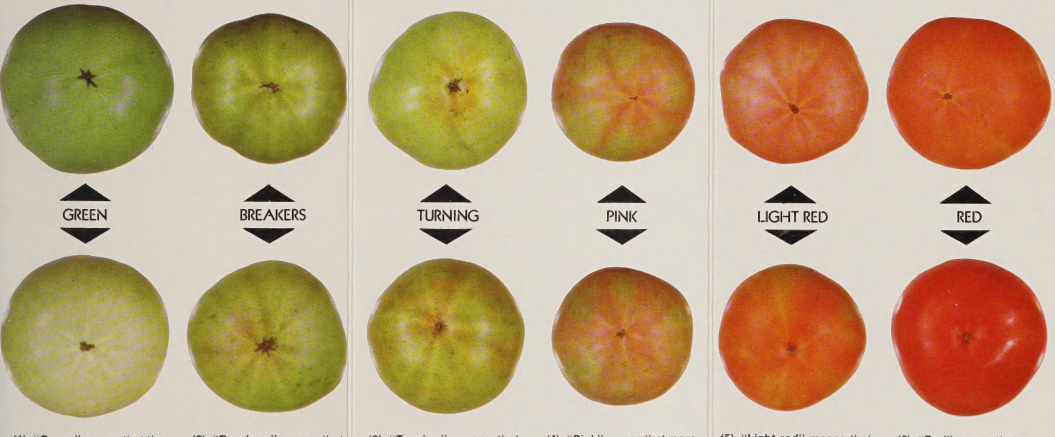
\includegraphics[width=0.85\textwidth]{images/imagem_usda1991.png}
    \label{fig:maturacao_usda}
    \legend{Fonte: \textcite{usda1991}.}
\end{figure}

Dois critérios desse padrão são determinantes para sistemas automatizados de classificação. Primeiramente a avaliação baseada na proporção de área atingida, em vez da média global de cor, e a transição de cor progressiva, na qual os estados iniciais admitem tonalidades amarelas, enquanto os finais exigem de forma predominante tons avermelhados e vermelhos. Para simplificar a rotulagem das amostras neste trabalho, os seis estados originais do USDA foram agrupados em três classes, sendo elas imaturo, intermediário e maduro. Embora \textcite{hou2024} também empreguem a fração de área vermelha como métrica, os autores adotam limiares de 80\% e 90\%, restringindo a classificação a frutos já avermelhados destinados ao consumo \textit{in natura}.

\subsection{Defeitos externos e calibre}

Os defeitos externos do tomate incluem rachaduras, podridões e mofos, danos mecânicos e manchas. Diferentemente da cor, os defeitos são padrões locais de textura e forma, de aparência muito variável, o que dificulta descrevê-los por regras explícitas \cite{dacosta2020}. Já o tamanho é uma grandeza geométrica. Para os tomates de mesa dos grupos redondo e oblongo, a classe é definida pelo maior diâmetro transversal \cite{ceagesp2003}; o tomate-cereja não segue esse mesmo critério de diâmetro, e por isso este trabalho mede o tamanho dos frutos, mas não os separa em classes de calibre. Em qualquer caso, medir o tamanho a partir da imagem exige converter medidas em pixels para milímetros.

% ----------------------------------------------------------
\section{Visão Computacional}
% ----------------------------------------------------------

Visão computacional é o conjunto de técnicas que extrai informações úteis de imagens digitais. Na inspeção de alimentos, ela permite realizar medições sem contato, não destrutivas e consistentes, substituindo aos poucos a inspeção visual humana, que é lenta, cansativa e subjetiva \cite{brosnan2004,cubero2011}. \textcite{chen2002} descrevem que um sistema de visão computacional para aplicações agrícolas é formado pela combinação de iluminação, câmera, placa de aquisição e software, em que o processamento consiste no realce da imagem, extração de características e classificação.

\subsection{Cor digital e balanço de branco}

Uma câmera digital registra, em cada pixel $(x,y)$, a resposta de três sensores, onde cada sensor representa um canal de cor: vermelho, verde e azul. No modelo físico de formação da imagem com iluminação uniforme, a resposta \(c_i(x,y)\) de cada canal \(i \in \{r, g, b\}\) depende do fator geométrico de sombreamento \(G(x,y)\), da reflectância espectral do objeto \(R_i(x,y)\) e da intensidade da fonte de luz \(L_{i}\) \cite{ebner2007}. Como uma mesma fruta fotografada sob diferentes condições de luz produz valores \acs{RGB} diferentes, torna-se necessário compensar o efeito da iluminação para que a cor medida represente fielmente o objeto \cite{ebner2007}.

Para transformar uma imagem capturada sob um iluminante \(L\) para um iluminante de referência \(L'\), o modelo diagonal de adaptação de von Kries aplica um fator de escala independente a cada canal de cor:
\[
\begin{bmatrix}
c_{r}^{\prime} \\
c_{g}^{\prime} \\
c_{b}^{\prime}
\end{bmatrix}
=
\begin{bmatrix}
k_{r} & 0 & 0 \\
0 & k_{g} & 0 \\
0 & 0 & k_{b}
\end{bmatrix}
\begin{bmatrix}
c_{r} \\
c_{g} \\
c_{b}
\end{bmatrix},
\qquad k_{i}=\frac{L_{i}^{\prime}}{L_{i}}
\]
Como o iluminante real \(L_{i}\) geralmente é desconhecido, a compensação exige obter uma estimativa \(\tilde{L}_i \approx L_i\) que permita normalizar cada canal da imagem e recuperar a reflectância do objeto (com o fator de sombreamento):
\[
\frac{c_{i}(x,y)}{\tilde{L}_{i}} = \frac{G(x,y)\,R_{i}(x,y)\,L_{i}}{\tilde{L}_{i}} \approx G(x,y)\,R_{i}(x,y)
\]
Em sistemas com iluminação controlada, como bancadas de inspeção visual, essa estimativa é obtida diretamente pela medição de uma superfície de referência branca sob a mesma fonte de luz \cite{ebner2007}. A partir dos valores registrados nessa referência, calcula-se um ganho por canal \(k_{i}\) para equilibrar as respostas e ajustar o branco medido a um valor neutro, corrigindo o balanço de branco de toda a cena.

\subsection{Segmentação e morfologia matemática}

A segmentação divide a imagem em regiões distintas, separando os pixels do objeto de interesse dos pixels do fundo \cite{gonzalez2010}. Quando o objeto apresenta alto contraste em relação a um fundo uniforme, a limiarização global define uma máscara binária a partir de um limiar de intensidade \(T\):
\[
B(x,y) =
\begin{cases}
1, & \text{se } f(x,y) > T, \\
0, & \text{caso contrário,}
\end{cases}
\]
em que \(f(x,y)\) representa a imagem em tons de cinza que será segmentada.

O método de \textcite{otsu1979} encontra o limiar ótimo \(T^{*}\) automaticamente a partir do histograma normalizado de \(L\) níveis de intensidade, com probabilidades \(p_k = n_k / N\) para \(k \in \{0, 1, \dots, L-1\}\), onde \(n_{k}\) é o número de pixels no nível \(k\) e \(N\) é o total de pixels. Para um limiar candidato \(t\), os pixels são divididos em duas classes, \(C_0\) (intensidades até \(t\)) e \(C_1\) (intensidades acima de \(t\)), com probabilidades acumuladas \(\omega_0(t)\) e \(\omega_1(t)\) e médias \(\mu_0(t)\) e \(\mu_1(t)\). O limiar ótimo maximiza a variância entre classes \(\sigma_B^2(t)\):
\[
\sigma_{B}^{2}(t) = \omega_{0}(t)\omega_{1}(t)\left[\mu_{1}(t)-\mu_{0}(t)\right]^{2},
\qquad T^{*} = \arg\max_{0 \le t < L-1} \sigma_{B}^{2}(t).
\]
Esse critério estatístico torna a escolha do limiar menos sensível a pequenas variações de iluminação entre as capturas.

Porém, na prática, a aplicação direta da limiarização é bastante afetada por ruídos de captura e reflexos. A filtragem passa-baixa prévia reduz o ruído antes do cálculo do limiar, enquanto operações de morfologia matemática refinam a máscara binária \(B\). As mais usadas são a abertura morfológica, que suaviza contornos e elimina pequenos ruídos isolados, e o fechamento morfológico, que une regiões fragmentadas e preenche falhas internas.

\subsection{Calibração geométrica e medição de tamanho}

Para medir em milímetros, é preciso conhecer a relação entre pixels e unidades reais no plano do objeto. A calibração de câmera usando um padrão plano de geometria conhecida, como um tabuleiro de xadrez, é um método clássico \cite{zhang2000}; os cantos do tabuleiro podem ser detectados com precisão subpixel e alta confiabilidade pelo detector de \textcite{duda2018}, disponível na biblioteca OpenCV. Como a lente e a perspectiva fazem a escala variar ao longo da imagem, uma alternativa simples à modelagem completa da câmera é estimar a escala localmente, em diferentes regiões da área de trabalho, a partir das distâncias conhecidas entre cantos vizinhos do tabuleiro. Essa simplificação tem uma limitação própria do modelo de câmera pinhole \cite{zhang2000}: a escala é válida para o plano do tabuleiro, enquanto o contorno visível do fruto está alguns milímetros acima dele, mais próximo da câmera, o que gera uma pequena superestimativa na medida.

\begin{figure}[H]
    \centering
    \caption{Exemplos de vistas de um padrão planar em diferentes orientações para calibração de câmera.}
    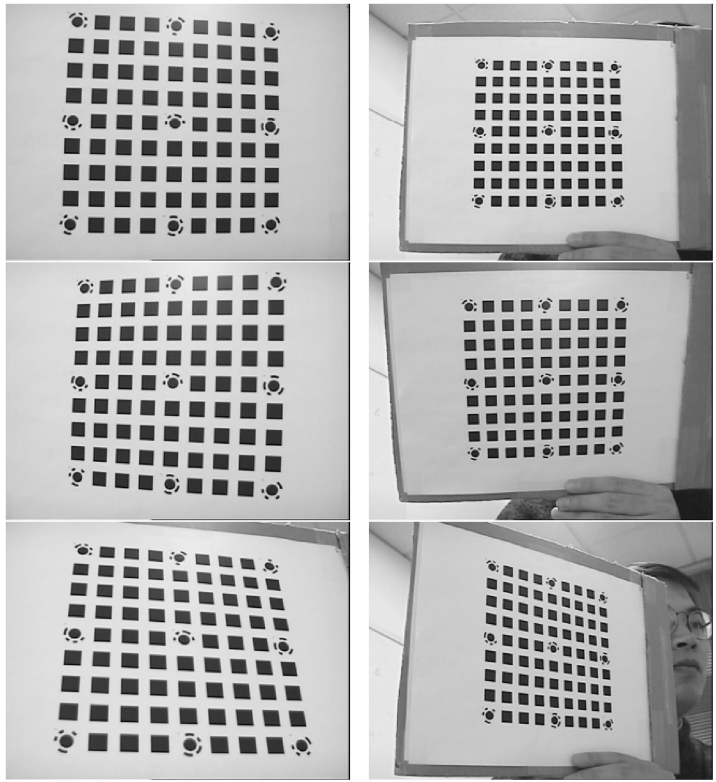
\includegraphics[width=0.85\textwidth]{images/imagem_zhang2000.png}
    \label{fig:calibracao_zhang2000}
    \legend{Fonte: Adaptado de \textcite{zhang2000}.}
\end{figure}

% ----------------------------------------------------------
\section{Classificação de Cor por Tabela de Consulta}
% ----------------------------------------------------------

Classificar cada pixel de uma imagem usando um modelo estatístico exige muito processamento para rodar em tempo real. Para resolver esse problema, utiliza-se uma tabela de consulta (\textit{lookup table}, LUT). Como uma imagem de 8 bits por canal possui \(256^3 \approx 16{,}7\) milhões de cores possíveis, o classificador pode ser avaliado uma única vez para todas elas, armazenando o resultado em uma tabela indexada pela própria cor. Assim, durante a execução, classificar um pixel passa a ser apenas uma leitura direta na memória.

\subsection{Agrupamento de cores com \textit{k-means}}

Rotular manualmente milhares de pixels para análise de cor é inviável na prática. Por isso, o algoritmo \textit{k-means} \cite{macqueen1967} resolve esse problema dividindo um conjunto de vetores de características \(\mathbf{x}_n \in \mathbb{R}^d\) (\(n = 1, \dots, N\)), onde cada \(\mathbf{x}_{n}\) representa os atributos de cor de um pixel, em \(k\) grupos distintos \(S_1, S_2, \dots, S_k\). O algoritmo busca minimizar a soma das distâncias ao quadrado entre cada ponto e o centro do seu grupo:
\[
J = \sum_{j=1}^{k} \sum_{\mathbf{x}_{n} \in S_{j}} \left\| \mathbf{x}_{n} - \boldsymbol{\mu}_{j} \right\|_{2}^{2},
\]
em que \(\boldsymbol{\mu}_{j}\) é o centroide do grupo \(S_{j}\) e \(\|\cdot\|_2\) representa a norma euclidiana. Na prática, o procedimento alterna entre atribuir cada pixel ao centroide mais próximo e recalcular a posição desses centroides até atingir a convergência.

Como a otimização de \(J\) é não convexa, o resultado final depende dos centros iniciais e pode convergir para mínimos locais. A inicialização \textit{k-means++} \cite{arthur2007} reduz esse problema escolhendo centros iniciais mais distantes entre si, de modo que pontos longe dos centros já selecionados tenham maior probabilidade de serem sorteados, tornando o agrupamento mais estável e consistente.

\subsection{Perceptron multicamadas}

O perceptron multicamadas (MLP) é uma rede neural com uma ou mais camadas ocultas de neurônios com função de ativação não linear, treinada pelo algoritmo de retropropagação do erro \cite{rumelhart1986}. Com neurônios ocultos suficientes, uma MLP consegue aproximar qualquer função contínua \cite{hornik1989}. Isso permite que ela aprenda fronteiras de decisão não lineares entre as classes de cor, ajustadas aos pixels rotulados, sem ficar presa às divisões rígidas que aconteceriam se cada cor fosse ligada apenas ao centro de grupo mais próximo. Os rótulos de treino vêm do agrupamento, mas a MLP permite unir vários grupos em uma mesma classe com uma fronteira contínua e ainda incluir a classe do fundo, que não entra na etapa de agrupamento.

A combinação entre MLP e LUT une a flexibilidade da rede com o baixo custo computacional da tabela. A principal limitação vem diretamente dos dados de treino: a tabela só é confiável para as cores observadas nas condições de iluminação da calibração, fazendo com que cores muito diferentes das vistas no treino recebam uma classificação estimada por extrapolação da rede.

% ----------------------------------------------------------
\section{Aprendizado Profundo e Redes Neurais Convolucionais}
% ----------------------------------------------------------

Defeitos como podridão, rachaduras e danos mecânicos são difíceis de descrever pela cor de pixels isolados: dependem de textura, forma e contexto espacial. O aprendizado profundo contorna essa dificuldade aprendendo as próprias características a partir dos dados, em múltiplos níveis de abstração \cite{lecun2015,goodfellow2016}. \textcite{kamilaris2018}, em uma revisão de 40 trabalhos de aplicação agrícola, observam que o aprendizado profundo superou, na maior parte deles, as técnicas de processamento de imagem comumente usadas.

\subsection{Redes neurais convolucionais}

As redes neurais convolucionais (\textit{convolutional neural networks}, CNN) são redes especializadas em imagens. Em vez de conectar cada pixel a cada neurônio, aplicam pequenos filtros que percorrem a imagem (convolução), compartilhando pesos e preservando a estrutura espacial \cite{lecun2015,goodfellow2016}. \textcite{zeiler2014} mostraram, ao visualizar redes treinadas, que as primeiras camadas respondem a bordas e manchas de cor e as seguintes a texturas e partes de objetos. Uma camada final, totalmente conectada, produz a pontuação de cada classe, convertida em probabilidades pela função \textit{softmax}. O trabalho de \textcite{krizhevsky2012} na competição ImageNet consolidou as CNN como o estado da arte em classificação de imagens.

Redes mais profundas, contudo, eram difíceis de otimizar: a partir de certa profundidade, o próprio erro de treinamento aumentava com o acréscimo de camadas. As redes residuais (ResNet) de \textcite{he2016} contornaram esse problema com conexões de atalho, que somam a entrada de um bloco à sua saída; assim, cada bloco aprende apenas uma correção residual em relação à identidade, o que facilita a otimização de redes profundas. Na ResNet, cada convolução é seguida de normalização em lote (\textit{batch normalization}) \cite{ioffe2015}, que estabiliza e acelera o treinamento. A ResNet-18, versão com 18 camadas \cite{he2016} e cerca de 11,7 milhões de parâmetros na implementação da biblioteca torchvision, é a menor da família, o que a torna adequada a conjuntos de dados pequenos e à execução em computadores sem placa de vídeo dedicada.

\subsection{Transferência de aprendizado}

Treinar uma CNN do zero exige grandes conjuntos de dados; com poucas centenas de imagens, a rede tende a memorizar os exemplos (sobreajuste). A transferência de aprendizado aproveita uma rede previamente treinada em um conjunto grande e genérico, como o ImageNet \cite{deng2009}, e a adapta à nova tarefa \cite{pan2010}. \textcite{yosinski2014} mostraram que as primeiras camadas de uma CNN aprendem características gerais, úteis para quase qualquer imagem, enquanto as últimas são específicas da tarefa original. Na prática, substitui-se a camada final por uma com o número de classes desejado e ajusta-se a rede inteira com taxa de aprendizado pequena (\textit{fine-tuning}), para não destruir as características já aprendidas. Em tomates, \textcite{dacosta2020} compararam o uso de ResNets pré-treinadas apenas como extratoras de características com o ajuste fino da rede na detecção de defeitos externos, em um conjunto de 43.843 imagens, e relatam vantagem do ajuste fino quando há dados suficientes.

\subsection{Aumento de dados e otimização}

O aumento de dados (\textit{data augmentation}) gera variações plausíveis das imagens de treino, como rotações, espelhamentos, recortes e pequenas alterações de brilho, ampliando artificialmente o conjunto e reduzindo o sobreajuste \cite{shorten2019}. As transformações devem respeitar a física do problema: um fruto pode aparecer em qualquer orientação, então rotações livres são válidas; já alterações fortes de cor seriam inadequadas para um sistema que usa a cor como critério e opera com iluminação calibrada.

O treinamento ajusta os pesos para minimizar uma função de perda, tipicamente a entropia cruzada, por descida de gradiente estocástica. O otimizador Adam \cite{kingma2015} adapta a taxa de aprendizado de cada peso a partir de estimativas dos momentos do gradiente; a variante AdamW \cite{loshchilov2019} aplica a penalização dos pesos (\textit{weight decay}) de forma desacoplada do gradiente, o que melhora a regularização. Em conjuntos desbalanceados, ponderar a perda de cada classe pelo inverso da sua frequência é uma forma usual de evitar que o classificador privilegie a classe majoritária \cite{he2009}.

% ----------------------------------------------------------
\section{Avaliação de Classificadores com Poucos Dados}
% ----------------------------------------------------------

Um classificador deve ser avaliado em dados que não participaram do treino. Com conjuntos pequenos, separar uma única parte para validação produz estimativas instáveis, que dependem de quais amostras caíram nessa parte. A validação cruzada em \(k\) partes (\textit{k-fold}) treina \(k\) modelos, cada um validado em uma parte diferente, e resume o desempenho pela média e pelo desvio padrão. \textcite{kohavi1995}, comparando métodos de estimativa em bases de dados reais, recomenda a validação cruzada estratificada, que mantém em cada parte a proporção das classes, com dez partes para a seleção de modelos; com poucas amostras da classe minoritária, porém, o número de partes fica limitado pela quantidade de exemplos dessa classe disponíveis para cada parte.

A independência entre treino e validação precisa ser garantida na unidade correta. Quando várias imagens provêm do mesmo fruto, elas são quase idênticas; se fotos do mesmo fruto aparecem em treino e validação, o modelo é avaliado em exemplos que praticamente já viu, e o desempenho é superestimado. \textcite{kapoor2023} identificam o vazamento de dados (\textit{data leakage}) como causa disseminada de resultados superestimados e irreprodutíveis em pesquisas baseadas em aprendizado de máquina. A solução é dividir os dados por grupo (no caso, por fruto), de modo que todas as imagens de um fruto fiquem do mesmo lado da divisão. Uma forma mais sutil de vazamento é escolher hiperparâmetros, como a época de parada do treinamento, com os mesmos dados usados para estimar o desempenho: a estimativa resultante é otimista \cite{cawley2010}, e uma estimativa não enviesada exige validação cruzada aninhada \cite{varma2006} ou um conjunto de teste independente.

As métricas também devem considerar o desbalanceamento. Tomando ``com defeito'' como classe positiva, a sensibilidade (\textit{recall}) mede a fração dos frutos defeituosos que o sistema detecta, e a especificidade, a fração dos sadios corretamente aceitos. A acurácia simples pode enganar quando uma classe predomina; a acurácia balanceada, média entre sensibilidade e especificidade, evita esse viés \cite{brodersen2010}. Com poucas amostras, convém relatar intervalos de confiança. O intervalo de \textcite{wilson1927} para proporções tem boa cobertura mesmo com amostras pequenas e proporções próximas de 0 ou 1, ao contrário do intervalo normal usual \cite{brown2001}. Como esses intervalos supõem observações independentes, o tamanho efetivo da amostra é o número de frutos, e não o de imagens; com poucas dezenas de frutos, as barras de erro da validação cruzada são necessariamente largas \cite{varoquaux2018}.

Por fim, redes neurais podem classificar com alta confiança exemplos muito diferentes dos vistos no treino \cite{nguyen2015}, e \textcite{hendrycks2017} mostram que a probabilidade da \textit{softmax}, embora útil como ponto de partida, é um indicador limitado para reconhecer essas entradas fora da distribuição de treino. Na prática, isso significa que o conjunto de treino precisa cobrir as variações que o sistema encontrará em operação (por exemplo, frutos em todos os estádios de maturação), e que o desempenho final deve ser medido em um conjunto de teste independente, coletado separadamente e avaliado uma única vez.

% ----------------------------------------------------------
\section{Trabalhos Relacionados}
% ----------------------------------------------------------

A classificação automática de frutos por visão computacional é estudada há mais de duas décadas, com uma transição visível de características extraídas manualmente para o aprendizado profundo.

Entre as abordagens baseadas em características manuais, \textcite{blasco2003} desenvolveram um sistema de inspeção em linha para laranjas, pêssegos e maçãs que estimava cor, tamanho, posição do pedúnculo e manchas, com precisão e repetibilidade semelhantes às da classificação manual. Para tomates-cereja, o sistema de Zhang \textit{et al.} (2009 \textit{apud} HOU \textit{et al.}, 2024) fotografava cada fruto de três ângulos e classificava a maturação em três níveis com análise de componentes principais e análise discriminante linear, alcançando 94,9\% de acerto em 414 frutos. \textcite{ireri2019} propuseram um sistema de visão para discriminação de defeitos e classificação de tomates a partir de imagens RGB, no qual a combinação de características de cor e textura obteve os melhores resultados e a acurácia diminuía à medida que aumentava o número de categorias de classificação.

Com o aprendizado profundo, \textcite{haggag2019} compararam CNN, redes neurais artificiais, mapas auto-organizáveis, quantização vetorial por aprendizado e máquinas de vetores de suporte, isoladas e combinadas, na separação de tomates imaturos, maduros e defeituosos; a combinação de CNN com rede neural artificial obteve o melhor resultado, com 90\% de acerto experimental entre maduros e defeituosos. \textcite{dacosta2020} construíram um conjunto de 43.843 imagens de tomates e treinaram classificadores ResNet para detectar defeitos externos, relatando que o modelo não confundia pedúnculo e cálice com defeitos. Mais recentemente, \textcite{hou2024} integraram, em um Raspberry Pi 4B com braço robótico, a medição de tamanho pelo contorno, a maturação por limiarização no espaço HSV (matiz, saturação e valor) e a detecção de defeitos com uma rede YOLOv8 (\textit{You Only Look Once}) modificada, relatando 99,1\% de acerto global na classificação de tomates de mesa em três graus (especial, primeiro e segundo) e capacidade de 1.350 tomates por hora.

Desses trabalhos, três observações orientam o presente estudo. Primeiro, cor, tamanho e defeito tendem a ser tratados por métodos distintos, cada um adequado à natureza do atributo: regras ou classificadores de cor para a maturação, geometria do contorno para o tamanho e redes profundas para os defeitos. Segundo, a transferência de aprendizado com ResNet foi empregada com sucesso na detecção de defeitos de tomate em um conjunto grande \cite{dacosta2020}; sua eficácia com cerca de uma centena de frutos, como neste trabalho, é justamente o que precisa ser verificado. Terceiro, os trabalhos relatam acurácias elevadas, mas nem sempre descrevem como os dados foram divididos: \textcite{hou2024}, por exemplo, treinam a detecção de defeitos com conjuntos públicos de imagens sem informar se a divisão entre treino e validação separa os frutos, aspecto decisivo quando há várias imagens por fruto \cite{kapoor2023}. O presente trabalho segue a linha de métodos especializados por atributo: classificação de cor por MLP convertida em LUT, medição de tamanho com escala calibrada por região e uma CNN ResNet-18 com transferência de aprendizado para defeitos, avaliada com divisão por fruto.
% ---

% ---
% 3 - Capítulo 3
% ---
% ----------------------------------------------------------
\chapter{Materiais e Métodos}\label{cap:metodos}
% ----------------------------------------------------------

Este capítulo descreve a bancada de aquisição, as calibrações, o processamento das imagens, a construção dos conjuntos de dados, o treinamento dos dois classificadores (a LUT de cor e a CNN de defeitos), a interface de operação e o protocolo de avaliação. Trata-se de uma pesquisa aplicada, de abordagem quantitativa e caráter experimental. A \autoref{fig:fluxo} resume o processamento de cada imagem: após o balanço de branco, os tomates são segmentados e, para cada um, são calculados o tamanho, a maturação e a probabilidade de defeito; a maturação e o defeito determinam o destino do fruto, e o tamanho é apenas medido e registrado.

\begin{figure}[htb]
	\caption{\label{fig:fluxo}Fluxo de processamento de uma imagem da bancada.}
	\centering
	\small
	\setlength{\fboxsep}{4pt}
	\fbox{Imagem da câmera} $\rightarrow$ \fbox{Balanço de branco} $\rightarrow$ \fbox{Segmentação (Otsu)} $\rightarrow$
	\fbox{\begin{tabular}{l}Tamanho e forma (escala por região)\\ Maturação (LUT de cor)\\ Defeito (CNN ResNet-18)\end{tabular}} $\rightarrow$ \fbox{Destino}
	\fonte{Elaborado pelo autor (2026).}
\end{figure}

O sistema foi implementado em Python, com a biblioteca OpenCV para o processamento de imagens e a inferência da CNN, a biblioteca scikit-learn para o \textit{k-means} e a MLP e o PyTorch para o treinamento da CNN. O código foi organizado em módulos pequenos e testáveis, com testes automatizados de unidade para a segmentação, a medição, a LUT, a inspeção e as métricas.

% ----------------------------------------------------------
\section{Bancada de Aquisição}
% ----------------------------------------------------------

A bancada consiste em uma caixa escura fechada, projetada para bloquear a luz ambiente, com a câmera fixa apontada para baixo a 303 mm do fundo (\autoref{fig:caixa}). Foi usada a câmera de um telefone celular, ligada ao computador pelo aplicativo DroidCam, com resolução de 1920 $\times$ 1080 pixels. O fundo é um tecido sintético preto e fosco, escolhido para contrastar com frutos de qualquer cor e para reduzir reflexos. Na imagem, apenas uma região de interesse retangular de 938 $\times$ 588 pixels (cerca de 188 $\times$ 118 mm) é processada; objetos que tocam a borda dessa região são descartados, pois parte deles não está visível.
% FIXME (autor): informar o modelo do celular e o custo aproximado dos componentes (celular, caixa, iluminação, computador), para sustentar o termo "baixo custo".
% FIXME (autor): descrever a iluminação usada (tipo de lâmpada/LED, posição, difusor) e se foco, exposição e balanço de branco da câmera foram travados no aplicativo.

\begin{figure}[htb]
	\caption{\label{fig:caixa}Caixa escura da bancada (modelo 3D).}
	\centering
	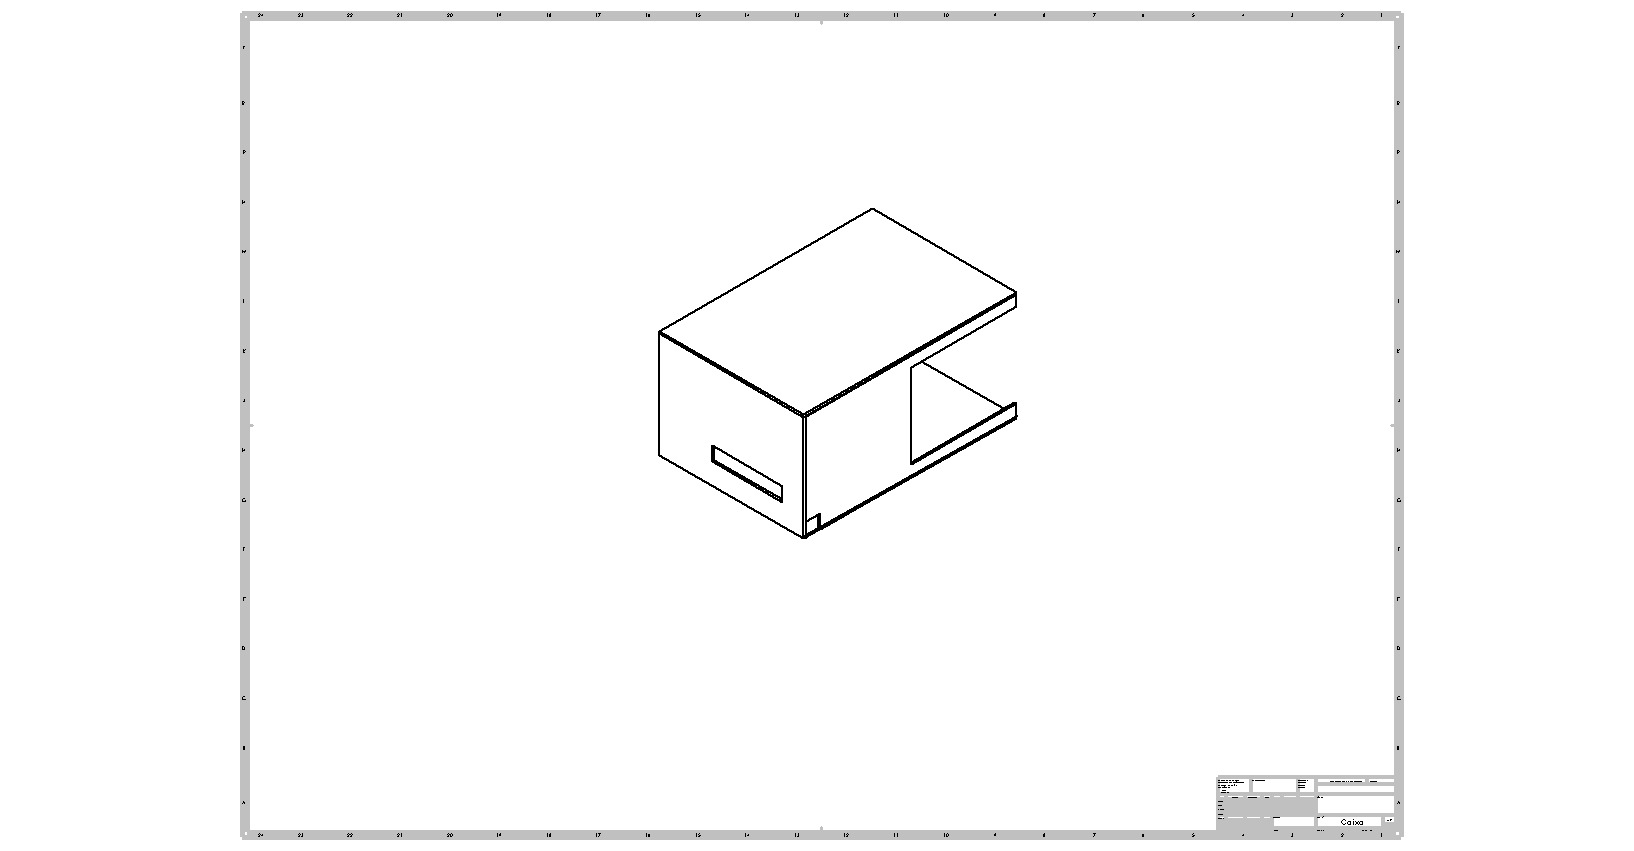
\includegraphics[width=0.85\textwidth]{images/caixa.jpg}
	\fonte{Elaborado pelo autor (2026).}
\end{figure}

% ----------------------------------------------------------
\section{Calibrações}
% ----------------------------------------------------------

\subsection{Balanço de branco}

Com uma folha branca na bancada, mede-se a média de cada canal na região de interesse e calcula-se um ganho por canal que leve essa média a um nível-alvo de 230, conforme o modelo diagonal de von Kries descrito no \autoref{cap:revisao}. Os ganhos obtidos foram 2,33 (R), 1,78 (G) e 1,48 (B): a luz da bancada era fria e a exposição, baixa, o que exigiu um ganho elevado no canal vermelho. O programa também mede a variação do branco ao longo da região, para detectar iluminação não uniforme; o canal vermelho variou 14,7\%, acima do limite de 8\% adotado como alerta, o que é discutido como limitação no \autoref{cap:resultados}. Todos os ganhos são aplicados a cada imagem antes de qualquer outro processamento, tanto no treinamento quanto na operação.

\subsection{Escala por região}

A escala foi calibrada com um tabuleiro de xadrez impresso com quadrados de 15 mm, colocado no plano do fundo. Os cantos internos foram detectados pelo método de \textcite{duda2018}, implementado no OpenCV. A região de interesse foi dividida em uma grade de 3 $\times$ 3 células e, em cada célula, a escala (mm/pixel) foi estimada como a média de 15 mm dividido pelo comprimento, em pixels, de cada segmento entre cantos vizinhos cujo ponto médio cai na célula. A \autoref{fig:escala} mostra o resultado: a escala variou de 0,1966 a 0,2038 mm/pixel, com média de 0,2008 mm/pixel, diminuindo de cima para baixo na imagem, padrão compatível com uma pequena inclinação da câmera em relação ao plano.

\begin{figure}[htb]
	\caption{\label{fig:escala}Calibração da escala por região com tabuleiro de 15 mm: escala (mm/pixel) e erro estimado em cada célula.}
	\centering
	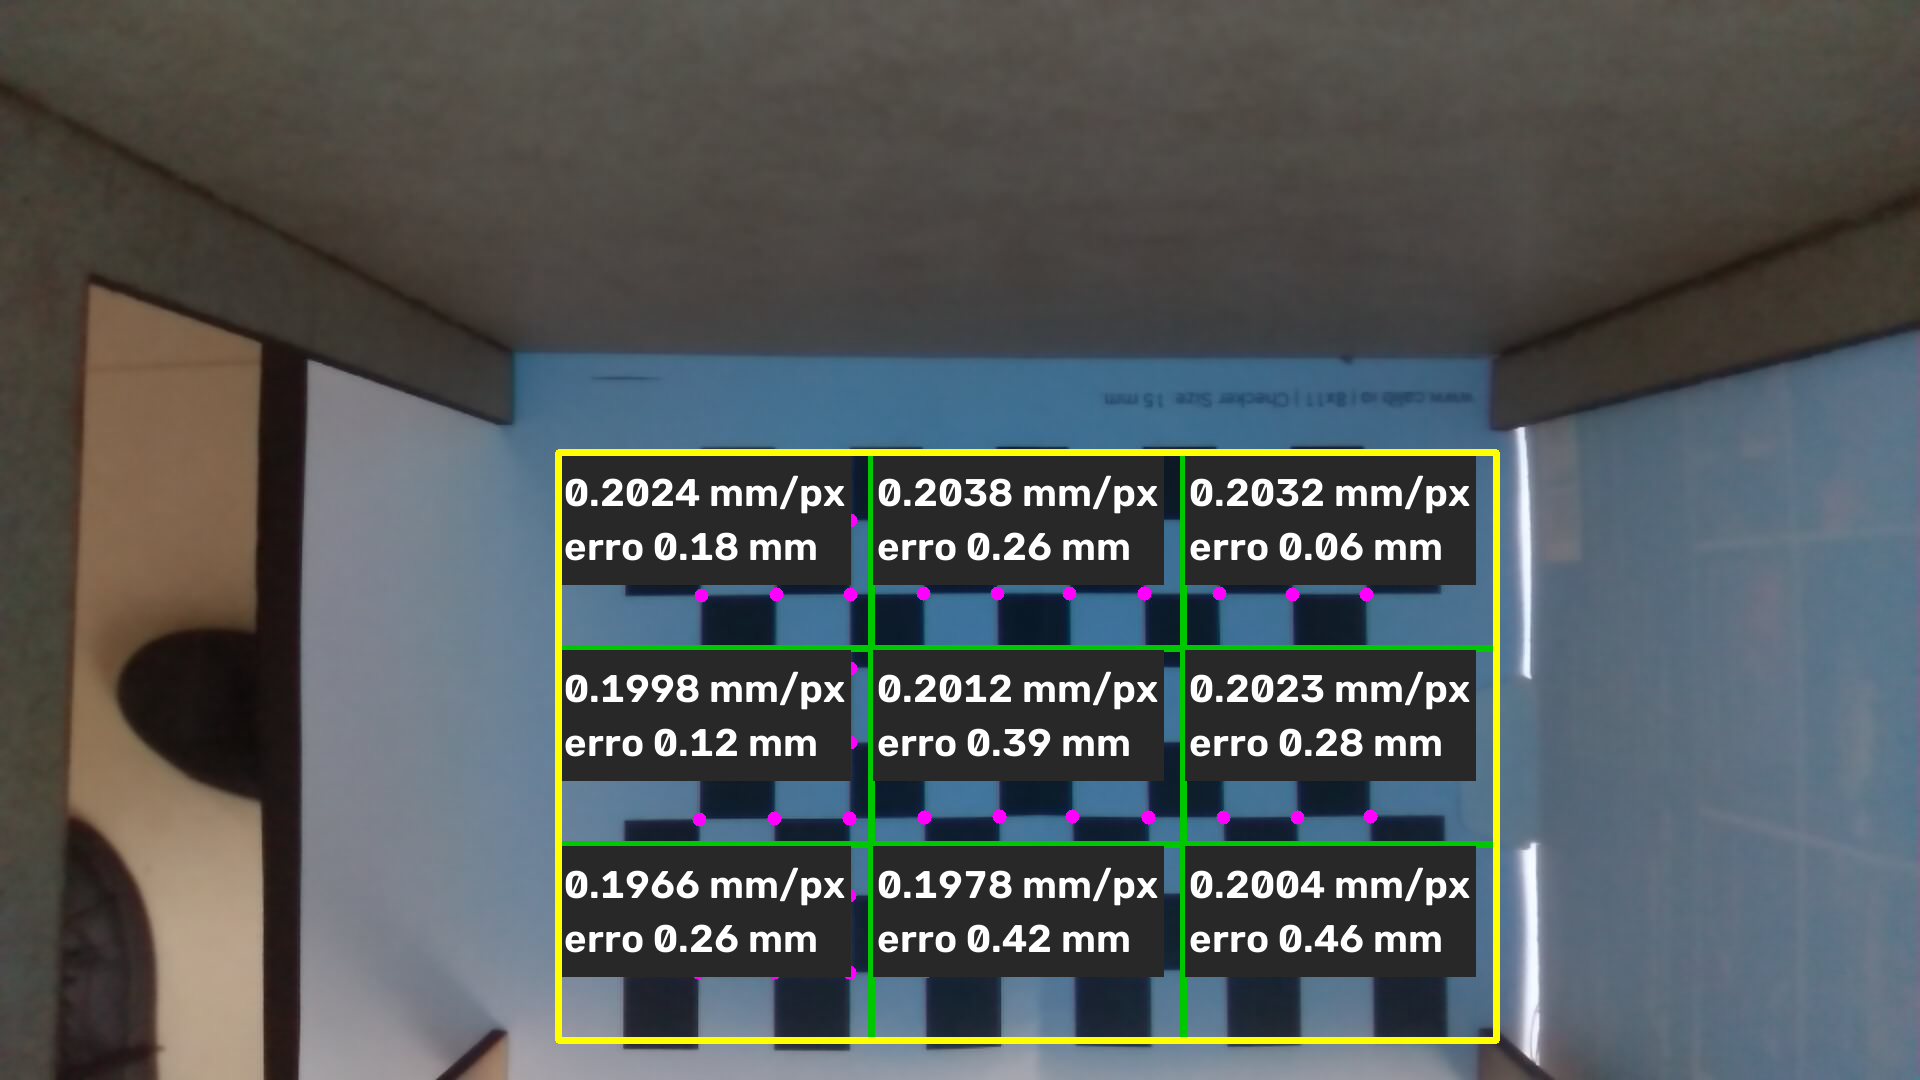
\includegraphics[width=0.9\textwidth]{images/bancada_escala.png}
	\fonte{Elaborado pelo autor (2026).}
\end{figure}

Para medir um objeto, cada um dos seus pixels é convertido em área (mm$^2$) com a escala da célula em que ele está, e o diâmetro equivalente é calculado a partir da área total. Assim, um objeto sobre a divisa entre células usa a escala de cada parte.

% ----------------------------------------------------------
\section{Segmentação e Medição}
% ----------------------------------------------------------

A segmentação segue o método descrito no \autoref{cap:revisao}. Na imagem com balanço de branco, calcula-se, para cada pixel, o maior valor entre os canais R, G e B, o que mantém contrastados contra o fundo preto tanto os frutos vermelhos quanto os verdes. Essa imagem é suavizada com filtro gaussiano de 5 $\times$ 5 pixels e limiarizada pelo método de Otsu. Em seguida, aplicam-se abertura (elemento estruturante elíptico de 5 pixels) e fechamento (9 pixels), e os contornos externos encontrados são preenchidos. Um objeto só é aceito se a diferença entre o seu brilho médio e o do fundo for de pelo menos 30 níveis; sem essa verificação, em uma imagem sem tomate o limiar de Otsu dividiria o próprio ruído do fundo em duas classes.

Para cada tomate segmentado, são calculados:
\begin{alineas}
	\item o diâmetro equivalente em milímetros, com a escala por região;
	\item o comprimento e a largura, dados pelos lados do menor retângulo girado que contém o contorno, multiplicados pela escala efetiva do fruto (raiz da razão entre a área em mm$^2$ e a área em pixels);
	\item a circularidade, $4\pi A/P^2$, em que $A$ é a área e $P$ o perímetro em pixels.
\end{alineas}

A medição foi validada com uma moeda de R\$ 1,00, de diâmetro nominal 27,00 mm, fotografada 64 vezes em todas as células da grade, com e sem a correção por região.

% ----------------------------------------------------------
\section{Conjuntos de Dados}
% ----------------------------------------------------------

Os tomates-cereja foram adquiridos em supermercado e fotografados na bancada com um programa de captura desenvolvido neste trabalho, que grava a foto e uma linha de rótulos em um arquivo CSV: número do tomate, defeitos presentes (rachado, podre ou mofado, dano mecânico e mancha) e estádio de maturação. Um tomate é considerado sadio quando não tem nenhum defeito marcado. O estádio de maturação é um campo opcional do programa; ele foi preenchido no conjunto de cor e no de teste, mas não nas sessões do conjunto de defeitos. Os rótulos foram atribuídos por inspeção visual do autor. Os tomates vieram de supermercado, e não diretamente de produtores, o que pode não representar a variedade de defeitos encontrada na origem. Foram formados três conjuntos, sempre com tomates distintos entre si:
% FIXME (autor): informar se algum defeito foi provocado (queda, pressão, imersão em água) ou se todos são naturais, e quantas compras/lotes foram usados.

\begin{alineas}
	\item \textbf{conjunto de cor}: 51 fotos (50 aproveitáveis) de 32 tomates com maturação informada (2 imaturos, 7 intermediários e 23 maduros), usado para gerar a LUT;
	\item \textbf{conjunto de defeitos}: 259 fotos aproveitáveis de 97 tomates, 49 sadios (140 fotos) e 48 com defeito (119 fotos), usado no treinamento e na validação cruzada da CNN. Das 266 fotos registradas na planilha de rótulos, 5 (de dois tomates) não tinham o arquivo de imagem correspondente e foram excluídas e 2 (de um mesmo tomate) foram descartadas porque o fruto não ficou inteiro dentro da região de interesse. Cerca de 40\% dos tomates foram fotografados em várias posições, girando o fruto entre as fotos (até 11 fotos por tomate); os demais têm uma foto. Entre os tomates com defeito, 25 têm mancha, 19 dano mecânico, 12 podridão ou mofo e 3 rachadura; 9 têm mais de um defeito;
	\item \textbf{conjunto de teste}: 22 tomates, uma foto cada, que não foram usados no treinamento de nenhum dos modelos, fotografados em 27/11/2026 logo após os últimos tomates do conjunto de defeitos: 9 sadios e 13 com defeito; 17 maduros, 4 intermediários e 1 imaturo.
\end{alineas}

Na primeira sessão de captura (tomates 1 a 29), todos os tomates sadios foram fotografados antes dos defeituosos. Como a ordem de captura pode se confundir com a classe (por exemplo, pelo aquecimento da câmera ou por pequenas mudanças de posição e de iluminação), as sessões seguintes e o conjunto de teste intercalaram, ao menos parcialmente, tomates sadios e defeituosos. A primeira sessão, porém, reúne 28 dos 97 tomates e 176 das 259 fotos do conjunto de defeitos, pois nela cada tomate foi fotografado várias vezes; o efeito dessa sessão é analisado no \autoref{cap:resultados}.

% ----------------------------------------------------------
\section{Classificação da Maturação por LUT}
% ----------------------------------------------------------

A LUT foi gerada em quatro etapas, conforme os fundamentos do \autoref{cap:revisao}:

\begin{alineas}
	\item \textbf{amostragem}: em cada foto do conjunto de cor, o tomate é segmentado e são sorteados até 4.000 pixels do seu interior (descartando uma faixa de 4 pixels junto à borda, onde a cor se mistura com o fundo) e 1.500 pixels do fundo;
	\item \textbf{agrupamento}: os pixels de tomate de todas as fotos, convertidos para L*a*b*, são agrupados em 8 grupos pelo \textit{k-means} com inicialização \textit{k-means++}. Um painel com a cor média e exemplos de cada grupo (\autoref{fig:grupos}) foi usado para dar nome a cada grupo entre verde, amarelado, rosado, vermelho e cálice;
	\item \textbf{treinamento da MLP}: uma MLP com duas camadas ocultas de 32 neurônios recebe as coordenadas L*a*b* normalizadas do pixel e prevê sua classe (as cores nomeadas mais o fundo). Para evitar que as classes mais frequentes dominem, cada classe contribui com até 20.000 pixels. Os pixels de cerca de 20\% dos tomates de cada maturação com pelo menos três tomates foram reservados para validação da MLP (sorteio por tomate); como o agrupamento usou todas as fotos, essa validação não é independente dos rótulos;
	\item \textbf{geração da tabela}: a MLP é avaliada uma única vez para as $256^3$ cores possíveis, e o resultado é gravado em uma tabela de 16,7 milhões de posições (cerca de 16 MB).
\end{alineas}

\begin{figure}[htb]
	\caption{\label{fig:grupos}Os oito grupos de cor do \textit{k-means}: cor média, fração dos pixels e exemplo de pixels de cada grupo.}
	\centering
	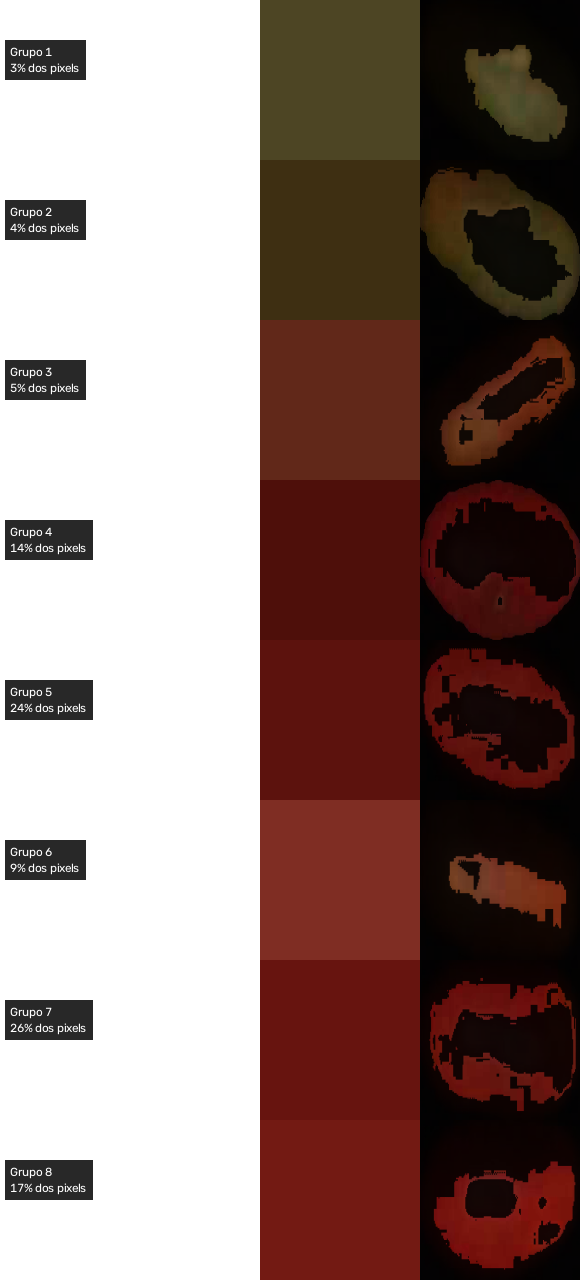
\includegraphics[height=0.55\textheight]{images/grupos_cor.png}
	\fonte{Elaborado pelo autor (2026).}
\end{figure}

Os grupos foram nomeados como verde (grupos 1 e 2), amarelado (3), rosado (6) e vermelho (4, 5, 7 e 8). Nenhum grupo correspondeu ao cálice, porque a segmentação e a amostragem do interior do fruto raramente o incluem.

Na operação, cada pixel do tomate é classificado por consulta à tabela, e a maturação é decidida pela proporção das cores, em uma adaptação dos estádios do USDA \cite{usda1991}:
\begin{alineas}
	\item \textbf{imaturo}: menos de 10\% da superfície colorida (amarelada, rosada ou vermelha), o que corresponde aos estádios verde e início de cor;
	\item \textbf{maduro}: mais de 60\% da superfície vermelha, correspondendo aos estádios vermelho claro e vermelho;
	\item \textbf{intermediário}: os demais casos (estádios virando e rosado).
\end{alineas}
Para o maduro, conta-se apenas o vermelho, e não qualquer cor, porque no padrão do USDA o amarelado caracteriza o início da mudança de cor; com a contagem de qualquer cor, um fruto inteiramente alaranjado seria classificado como maduro.

% ----------------------------------------------------------
\section{Detecção de Defeitos por CNN}
% ----------------------------------------------------------

\subsection{Entrada e arquitetura}

A entrada da CNN é um recorte quadrado em torno do tomate segmentado, com margem de 15\% do seu maior lado, redimensionado para 224 $\times$ 224 pixels, na imagem com balanço de branco. O fundo do recorte não é mascarado, pois a borda do fruto, onde costumam estar rachaduras e danos, poderia ser cortada por uma máscara imperfeita. A rede é uma ResNet-18 \cite{he2016} com os pesos pré-treinados no ImageNet \cite{deng2009}, cuja camada final foi substituída por uma camada totalmente conectada de duas saídas (sadio e com defeito). A normalização da entrada pela média e pelo desvio padrão do ImageNet foi incorporada ao próprio modelo, para que o programa de operação não precise reproduzi-la.

\subsection{Treinamento}

Toda a rede foi ajustada (\textit{fine-tuning}) com o otimizador AdamW \cite{loshchilov2019}, taxa de aprendizado de $10^{-4}$, penalização dos pesos de $10^{-4}$ e lotes de 16 imagens, minimizando a entropia cruzada ponderada pelo inverso da frequência de cada classe \cite{he2009}. O aumento de dados aplicou, a cada época, rotação aleatória de até 180$^\circ$, espelhamentos horizontal e vertical, recorte aleatório de 80\% a 100\% da área e pequenas variações de brilho, contraste e saturação (até 15\%, 15\% e 10\%). A matiz não foi alterada, para preservar a cor do fruto.

\subsection{Validação cruzada e modelo final}

O desempenho esperado em tomates novos foi estimado por validação cruzada em 5 partes, com divisão \emph{por tomate} e estratificada por classe (\textit{StratifiedGroupKFold}): todas as fotos de um tomate ficam na mesma parte, evitando o vazamento descrito por \textcite{kapoor2023}. Em cada parte, uma rede nova foi treinada por até 30 épocas, e a época com a maior acurácia balanceada na validação (com desempate pela menor perda) foi registrada. Como essa escolha usa os próprios dados de validação, a estimativa resultante é otimista \cite{cawley2010}, razão pela qual o desempenho final é medido no conjunto de teste. As métricas da validação cruzada são calculadas por foto; como um tomate pode ter até 11 fotos, os tomates muito fotografados pesam mais nessas médias.

O modelo final foi treinado com todos os tomates do conjunto de defeitos pelo número de épocas igual à mediana das melhores épocas das 5 partes. Separar tomates apenas para escolher a época retiraria exemplos de defeito, que são escassos. O modelo foi exportado no formato ONNX, com a função \textit{softmax} na saída, e é executado na operação pelo módulo de redes neurais do OpenCV, sem necessidade do PyTorch ou de placa de vídeo. Após a exportação, conferiu-se que as probabilidades calculadas pelo OpenCV coincidem com as do PyTorch em todas as imagens de treino (diferença máxima tolerada de 0,02). Um tomate é classificado como defeituoso quando a probabilidade de defeito é de pelo menos 0,5.

O treinamento foi executado em um computador com placa de vídeo NVIDIA GeForce RTX 3050.

% ----------------------------------------------------------
\section{Interface de Operação}
% ----------------------------------------------------------

A interface homem-máquina (IHM) foi desenvolvida com a biblioteca Tkinter. Ela mostra o vídeo da câmera restrito à região de interesse e, ao comando do operador (botão ou barra de espaço) ou em modo contínuo, inspeciona a imagem: cada tomate é contornado na cor do seu destino e numerado, e um cartão lateral apresenta, para cada fruto, o destino, a maturação com as porcentagens de superfície colorida e vermelha, a probabilidade de defeito, o diâmetro, o comprimento, a largura e a circularidade. Contadores mostram quantos frutos foram enviados a cada destino, e cada inspeção é registrada em um arquivo CSV diário.

O destino é decidido em duas etapas: um tomate com defeito vai para o descarte, qualquer que seja a sua cor; os demais são separados pela maturação (imaturo, intermediário ou maduro). Internamente, a inspeção completa de uma imagem é oferecida à interface por uma única classe (padrão de projeto \textit{Facade}), que encadeia balanço de branco, segmentação, medição, LUT e CNN; com isso, a mesma rotina é usada pela IHM e pela avaliação no conjunto de teste.

% ----------------------------------------------------------
\section{Protocolo de Avaliação}
% ----------------------------------------------------------

O conjunto de teste foi processado uma única vez, depois de concluídos a LUT e o modelo final da CNN, pela mesma rotina de inspeção da IHM, sem nenhum ajuste posterior de limiares ou modelos; a versão preliminar da CNN, treinada com 28 tomates, nunca foi aplicada a ele. Em cada foto, se mais de um objeto fosse segmentado, o maior seria tomado como o tomate. Foram calculados:

\begin{alineas}
	\item para a CNN, tomando ``com defeito'' como classe positiva: acurácia, sensibilidade, especificidade, acurácia balanceada, precisão e F1, além da matriz de confusão;
	\item para a LUT: a acurácia da maturação nas três classes e a matriz de confusão, em todos os tomates, com ou sem defeito;
	\item para o sistema completo: a acurácia do destino final, sendo esperado o descarte para os tomates com defeito e a classe de maturação rotulada para os sadios;
	\item o tempo de processamento por imagem, desde o balanço de branco até a decisão do destino.
\end{alineas}

A unidade de análise é o tomate. Para as proporções (acurácia, sensibilidade e especificidade), foram calculados intervalos de confiança de 95\% pelo método de \textcite{wilson1927}. Os critérios de aceitação definidos no início do projeto foram: segmentação correta em pelo menos 95\% das imagens; erro de até 0,5 mm na calibração da escala, medido pelo resíduo das distâncias entre cantos do próprio tabuleiro; erro médio absoluto de até 1 mm no diâmetro; acurácia de pelo menos 90\% na maturação; F1 de pelo menos 0,85 na classe ``com defeito''; e tempo de processamento de até 200 ms por tomate.

% ---

% ---
% 4 - Conclusão
% ---
%\phantompart
% ----------------------------------------------------------
\chapter{Resultados e Discussão}\label{cap:resultados}
% ----------------------------------------------------------

Este capítulo apresenta os resultados na ordem do processamento: calibração e medição, segmentação, classificação da maturação, detecção de defeitos e desempenho do sistema completo no conjunto de teste. Ao final, os resultados são comparados com os critérios de aceitação e as limitações do estudo são discutidas.

% ----------------------------------------------------------
\section{Calibração e Medição de Tamanho}
% ----------------------------------------------------------

A calibração de escala (\autoref{fig:escala}) apresentou resíduo máximo de 0,46 mm, na célula inferior direita, dentro do limite de 0,5 mm; por ser calculado com o próprio tabuleiro, esse resíduo mede a consistência da calibração, e não a exatidão em outros objetos, avaliada a seguir com a moeda. A escala variou 3,6\% entre a maior e a menor célula, e cerca de 2,4\% entre as médias da linha superior e da inferior. Uma variação gradual e aproximadamente linear desse tipo é típico de uma câmera ligeiramente inclinada em relação ao plano, e não de distorção da lente, que seria simétrica em torno do centro da imagem.

A \autoref{tab:moeda} resume as 64 medições da moeda de 27,00 mm distribuídas pelas nove células. A correção por região reduziu o desvio padrão das medidas quase pela metade (de 0,32 para 0,17 mm), isto é, tornou a medida menos dependente da posição do objeto na imagem, e o erro médio absoluto de 0,45 mm ficou abaixo do limite de 1 mm. Em uma mesma posição, sem reposicionar a moeda, o desvio padrão foi de 0,01 a 0,03 mm; esse valor mede o ruído da câmera e da segmentação, e não a repetibilidade de posicionamento. Como as medições repetidas na mesma posição não são independentes, a estatística por posição (uma média para cada uma das dez primeiras posições) também foi calculada e deu resultado semelhante: erro médio absoluto de 0,53 mm com correção.

\begin{table}[htb]
	\ABNTEXfontereduzida
	\centering
	\caption{\label{tab:moeda}Erro na medição do diâmetro de uma moeda de 27,00 mm (64 medições em todas as células).}
	\begin{tabular}{lccccc}
		\toprule
		Escala & Erro médio & Desvio padrão & Erro médio absoluto & RMSE & Faixa do erro \\
		 & (mm) & (mm) & (mm) & (mm) & (mm) \\
		\midrule
		Única (média) & $-0{,}48$ & 0,32 & 0,49 & 0,57 & $-1{,}16$ a $+0{,}11$ \\
		Por região & $-0{,}45$ & 0,17 & 0,45 & 0,48 & $-0{,}82$ a $-0{,}21$ \\
		\bottomrule
	\end{tabular}
	\fonte{Elaborado pelo autor (2026).}
\end{table}

A correção por região, porém, não removeu o viés: todas as medições com correção ficaram abaixo do valor real, em média 0,45 mm. As causas foram investigadas. A segmentação não corta a borda da moeda: no perfil de brilho radial, o contorno segmentado ficou 0,7 pixel por fora da borda, o que aumentaria a medida. A espessura da moeda, cerca de 2 mm mais próxima da câmera, também aumentaria a medida (cerca de 0,7\%). O tamanho dos quadrados impressos do tabuleiro foi conferido. A explicação mais provável é que o tabuleiro e a moeda não estivessem exatamente no mesmo plano (por exemplo, por diferença de altura ou inclinação do papel sobre o tecido), o que é coerente com a limitação do modelo \textit{pinhole} discutida no \autoref{cap:revisao}. Essa hipótese não foi testada. Um fator de correção calculado com essas mesmas medições não foi aplicado, pois o sistema seria validado com os dados usados para ajustá-lo.

Nos tomates, a medição não pôde ser validada, pois o diâmetro com paquímetro não foi registrado nos rótulos. No conjunto de teste, os diâmetros equivalentes medidos variaram de 18,9 a 32,2 mm (mediana de 26,2 mm) e a circularidade de 0,51 a 0,86 (mediana de 0,79). A circularidade ficou bem abaixo da da moeda (0,91 a 0,92). O alongamento explica só parte disso: uma elipse com razão de 1,5 entre os eixos ainda tem circularidade de cerca de 0,94, e o tomate 11, com razão de 1,3, teve circularidade de 0,51. Os valores baixos refletem principalmente irregularidades do contorno, como defeitos, cálice e ruído da segmentação, que aumentam o perímetro.

% ----------------------------------------------------------
\section{Segmentação}
% ----------------------------------------------------------

A segmentação encontrou um único objeto em cada uma das 22 fotos do conjunto de teste, sem objetos espúrios. No tomate 16, porém, o objeto segmentado tem 47,9 mm de comprimento por 22,0 mm de largura, com um estreitamento no meio, o que sugere dois frutos encostados segmentados como um só; se for o caso, a segmentação acertou 21 das 22 fotos. No conjunto de defeitos, apenas as 2 fotos de um tomate que não estava inteiramente dentro da região de interesse foram rejeitadas, como previsto. O uso do maior canal de cor, em vez do nível de cinza, foi decisivo durante o desenvolvimento: com o nível de cinza, um tomate vermelho-escuro ficava abaixo do contraste mínimo, e a presença de um objeto branco na região deslocava o limiar de Otsu a ponto de perder os tomates.

As imagens da bancada, contudo, são escuras (\autoref{fig:testeexemplos}): mesmo após o balanço de branco, os frutos aparecem com pouco brilho sobre o fundo preto, o que se deve à iluminação fraca já indicada pelos ganhos elevados na calibração de branco.

% ----------------------------------------------------------
\section{Classificação da Maturação}
% ----------------------------------------------------------

\subsection{Validação da LUT}

No nível do pixel, segundo o registro de execução do programa, a MLP acertou 99,7\% dos pixels dos tomates reservados para validação. Esse número, entretanto, é pouco informativo: os rótulos dos pixels vêm dos grupos do \textit{k-means}, que foram calculados com todas as fotos, inclusive as de validação, e os tomates de validação não incluíam nenhum imaturo, pois havia apenas dois tomates imaturos no conjunto de cor.

Aplicada às 50 fotos aproveitáveis do conjunto de cor, a regra de maturação acertou 62\% tanto nos tomates de validação (5 de 8 fotos) quanto nos de treino (26 de 42 fotos). Todos os erros foram de tomates rotulados como intermediários e classificados como maduros: 16 das 19 fotos de intermediários usadas no treino tinham mais de 60\% da superfície classificada como vermelha. A causa principal está nos próprios grupos de cor. O grupo nomeado rosado tem praticamente a mesma matiz dos grupos vermelhos (ângulo de cerca de 36$^\circ$ no plano a*b*, contra 34$^\circ$ a 37$^\circ$) e difere deles apenas por ser mais claro; todos os grupos têm luminosidade baixa (L* entre 16 e 31). Assim, a separação entre rosado e vermelho depende do brilho, e não da cor, e com a iluminação fraca da bancada a maior parte da superfície de um fruto rosado é classificada como vermelha. Contribui também a subjetividade do rótulo: a fronteira entre os estádios rosado e vermelho claro do USDA é estreita, e o rótulo foi atribuído visualmente.

\subsection{Conjunto de teste}

No conjunto de teste, a maturação foi classificada corretamente em 19 dos 22 tomates (86,4\%; IC 95\%: 66,7\% a 95,3\%), conforme a \autoref{tab:maturacao}. Esse valor, porém, é dominado pelos tomates maduros, que formam 17 dos 22 frutos e foram todos acertados. Nas classes minoritárias, o desempenho foi baixo: 2 de 4 intermediários e nenhum dos imaturos (havia apenas um). Um dos intermediários acertados (tomate 14) teve 59,9\% da superfície vermelha, praticamente sobre o limite de 60\%. Os dois intermediários errados tinham 91\% da superfície classificada como vermelha, repetindo o padrão observado no conjunto de cor. O tomate imaturo (\autoref{fig:testeexemplos}d), esverdeado com regiões alaranjadas, teve 83\% da superfície classificada como colorida (25\% como vermelha), muito acima do limite de 10\% para imaturo, e foi classificado como intermediário: os grupos nomeados como verde reúnem apenas 6\% dos pixels de treino, e os tons verde-amarelados escuros desse fruto foram atribuídos a classes coloridas. A média das taxas de acerto por classe é de apenas 50\%, o que mostra que a acurácia global superestima a capacidade da LUT de distinguir os estádios.

\begin{table}[htb]
	\centering
	\caption{\label{tab:maturacao}Matriz de confusão da maturação no conjunto de teste (22 tomates).}
	\begin{tabular}{lccc}
		\toprule
		Real $\backslash$ LUT & Imaturo & Intermediário & Maduro \\
		\midrule
		Imaturo & 0 & 1 & 0 \\
		Intermediário & 0 & 2 & 2 \\
		Maduro & 0 & 0 & 17 \\
		\bottomrule
	\end{tabular}
	\fonte{Elaborado pelo autor (2026).}
\end{table}

Assim, o critério de 90\% de acurácia na maturação não foi atingido, e a LUT, na forma atual, separa bem os frutos maduros, mas não distingue com confiabilidade os estádios intermediários. As causas identificadas são os grupos de cor que separam rosado e vermelho pelo brilho, a pouca quantidade de tomates imaturos e intermediários no conjunto de cor, a iluminação fraca, que exige ganho alto no canal vermelho, e a subjetividade dos rótulos.

% ----------------------------------------------------------
\section{Detecção de Defeitos}
% ----------------------------------------------------------

\subsection{Validação cruzada}

A \autoref{tab:cnncv} apresenta a validação cruzada da CNN em 5 partes, com divisão por tomate e métricas calculadas por foto. A acurácia balanceada média foi de 93,6\% $\pm$ 1,9\% (desvio padrão populacional entre as partes), com sensibilidade de 95,0\% e especificidade de 92,1\%. Somando as partes, 113 das 119 fotos de tomates com defeito foram detectadas, e 11 das 140 fotos de tomates sadios foram classificadas como defeituosas.

\begin{table}[htb]
	\ABNTEXfontereduzida
	\centering
	\caption{\label{tab:cnncv}Validação cruzada da CNN em 5 partes, com divisão por tomate (métricas por foto).}
	\begin{tabular}{cccccc}
		\toprule
		Parte & Melhor época & Acurácia & Acur. balanceada & Sensibilidade & Especificidade \\
		\midrule
		1 & 24 & 90,4\% & 90,5\% & 91,7\% & 89,3\% \\
		2 & 22 & 96,2\% & 96,1\% & 95,8\% & 96,4\% \\
		3 & 28 & 94,2\% & 94,3\% & 95,8\% & 92,9\% \\
		4 & 8 & 94,2\% & 94,3\% & 95,8\% & 92,9\% \\
		5 & 30 & 92,2\% & 92,5\% & 95,7\% & 89,3\% \\
		\midrule
		Média & -- & 93,4\% & 93,6\% & 95,0\% & 92,1\% \\
		Desvio padrão & -- & 2,0\% & 1,9\% & 1,7\% & 2,7\% \\
		\bottomrule
	\end{tabular}
	\fonte{Elaborado pelo autor (2026).}
\end{table}

As curvas de aprendizado (\autoref{fig:curvas}) mostram a perda de treino diminuindo de forma contínua, enquanto a perda de validação oscila bastante de uma época para a outra, comportamento esperado com cerca de 50 fotos de validação por parte, em que poucas imagens mudam a métrica. A melhor época variou de 8 a 30 entre as partes, e o modelo final foi treinado por 24 épocas (a mediana). Na parte 5, a melhor época coincidiu com o limite de 30, o que indica que um limite maior poderia ter sido testado. Em uma versão preliminar, treinada com apenas 28 tomates, a validação cruzada havia resultado em 94,5\% $\pm$ 3,7\%.

A média da validação cruzada, porém, é dominada pela primeira sessão de captura, em que todos os sadios foram fotografados antes dos defeituosos e que responde por 176 das 259 fotos. Separando os erros por sessão, a primeira teve especificidade de 96,1\% (98 de 102 fotos de sadios) e sensibilidade de 94,6\% (70 de 74), enquanto as sessões seguintes, com classes intercaladas, tiveram especificidade de apenas 81,6\% (31 de 38) e sensibilidade de 95,6\% (43 de 45), com acurácia balanceada de cerca de 88,6\%. Não é possível afirmar que a rede tenha aprendido características da sessão, e não do fruto, mas a diferença é compatível com isso, e o fundo não mascarado do recorte tornaria esse aprendizado possível.

\begin{figure}[htb]
	\caption{\label{fig:curvas}Curvas de aprendizado de duas partes da validação cruzada: perda de treino (azul) e de validação (vermelho), normalizadas pela perda máxima, e acurácia balanceada de validação (verde). A linha vertical marca a melhor época.}
	\centering
	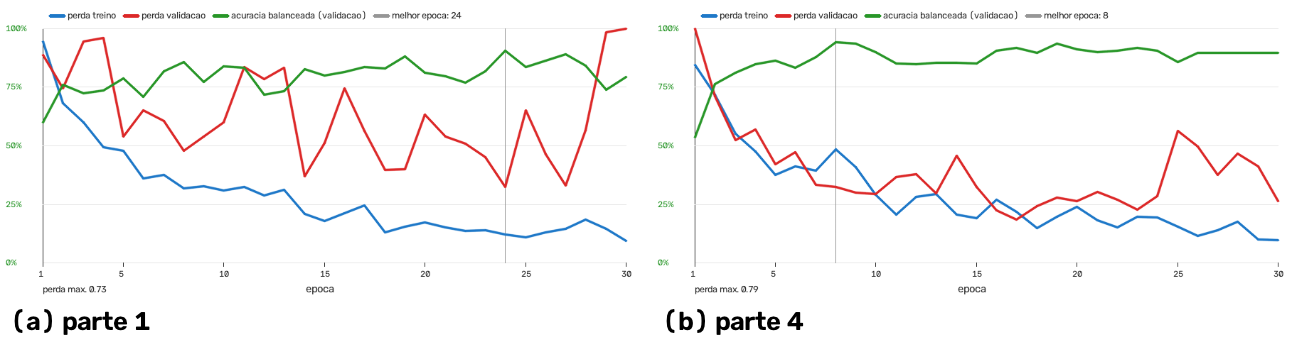
\includegraphics[width=\textwidth]{images/curvas_cnn.png}
	\fonte{Elaborado pelo autor (2026).}
\end{figure}

O modelo exportado em ONNX e executado pelo OpenCV reproduziu as probabilidades do PyTorch com diferença máxima de 0,0013 (registrada no arquivo de execução do treino), confirmando que a interface usa o mesmo modelo avaliado.

\subsection{Conjunto de teste}

No conjunto de teste (\autoref{tab:cnnteste}), a CNN classificou corretamente 19 dos 22 tomates (86,4\%), com sensibilidade de 84,6\% (11 de 13 defeituosos detectados) e especificidade de 88,9\% (8 de 9 sadios aceitos), precisão de 91,7\% e F1 de 0,88. Por reamostragem (\textit{bootstrap}, 20.000 amostras) dos 22 tomates, o intervalo de 95\% do F1 vai de 0,71 a 1,00, e 33\% das reamostras ficam abaixo de 0,85. O resultado de cada tomate está no \autoref{ap:teste}.

\begin{table}[htb]
	\centering
	\caption{\label{tab:cnnteste}Desempenho da CNN no conjunto de teste (22 tomates, uma foto cada), com intervalos de confiança de Wilson (95\%).}
	\begin{tabular}{lcc}
		\toprule
		Métrica & Valor & IC 95\% \\
		\midrule
		Acurácia & 86,4\% (19/22) & 66,7\% a 95,3\% \\
		Sensibilidade & 84,6\% (11/13) & 57,8\% a 95,7\% \\
		Especificidade & 88,9\% (8/9) & 56,5\% a 98,0\% \\
		Acurácia balanceada & 86,8\% & -- \\
		F1 (classe com defeito) & 0,88 & 0,71 a 1,00 (\textit{bootstrap}) \\
		\bottomrule
	\end{tabular}
	\fonte{Elaborado pelo autor (2026).}
\end{table}

Os três erros estão ilustrados na \autoref{fig:testeexemplos}. Os dois defeitos não detectados foram uma mancha (tomate 7, probabilidade de defeito de 0,03) e um dano mecânico (tomate 22, probabilidade de 0,19), defeitos pequenos e de baixo contraste nas imagens escuras da bancada. O tomate sadio descartado (tomate 16, probabilidade de 0,72) é o objeto alongado discutido na seção de segmentação, possivelmente dois frutos encostados. Em qualquer caso, é uma imagem atípica em relação às de treino, e o erro é possivelmente relacionado à dificuldade das redes com entradas afastadas da distribuição de treino \cite{nguyen2015,hendrycks2017}.
% FIXME (autor): conferir na foto original se o tomate 16 é um único fruto alongado ou dois frutos encostados.

\begin{figure}[htb]
	\caption{\label{fig:testeexemplos}Exemplos do conjunto de teste, como exibidos pela IHM: o contorno tem a cor do destino decidido pelo sistema.}
	\centering
	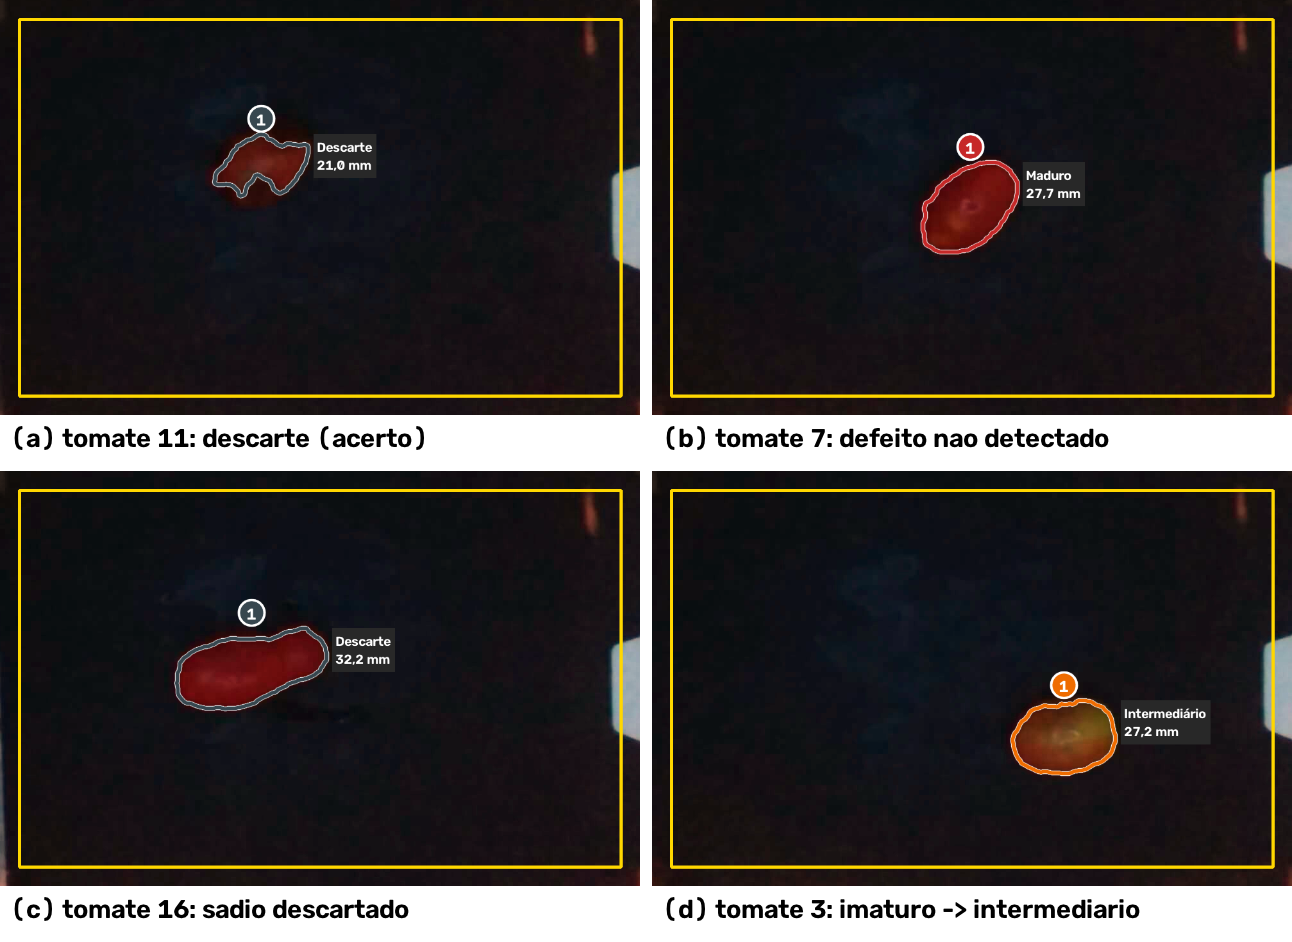
\includegraphics[width=\textwidth]{images/teste_exemplos.png}
	\fonte{Elaborado pelo autor (2026).}
\end{figure}

A acurácia balanceada no teste (86,8\%) ficou abaixo da média da validação cruzada (93,6\%), mas próxima da obtida nas sessões de captura intercaladas (cerca de 88,6\%). Três fatores contribuem para a diferença: o peso da primeira sessão na validação cruzada, discutido acima; a escolha da época de parada com os próprios dados de validação, que torna a validação cruzada otimista \cite{cawley2010}; e o tamanho do teste, em que um único erro muda a sensibilidade em 7,7 pontos percentuais e a especificidade em 11,1. O F1 de 0,88 atende ao critério de 0,85 na estimativa pontual, mas o intervalo de 0,71 a 1,00 e o limite inferior da sensibilidade (57,8\%) mostram que essa conclusão ainda é frágil.

% ----------------------------------------------------------
\section{Sistema Completo}
% ----------------------------------------------------------

Combinando a CNN e a LUT, o destino final foi correto em 18 dos 22 tomates do teste (81,8\%; IC 95\%: 61,5\% a 92,7\%). Dos quatro erros, dois são defeituosos que seriam enviados ao mercado como maduros (tomates 7 e 22), o erro de maior custo para o produtor; um é um tomate sadio descartado (tomate 16); e um é um imaturo enviado como intermediário (tomate 3). Os dois intermediários classificados como maduros pela LUT não afetaram o destino, porque ambos tinham defeito e foram corretamente descartados.

O tempo de processamento de uma imagem, do balanço de branco à decisão do destino, teve mediana de 53,5 ms (de 50,7 a 56,7 ms) no computador de desenvolvimento, com a CNN executada pelo OpenCV na CPU e as fotos lidas do disco, isto é, sem incluir a captura pela câmera. O valor está bem abaixo da meta de 200 ms por tomate e corresponde a cerca de 19 imagens por segundo.
% FIXME (autor): informar o processador e a memória do computador de desenvolvimento. A primeira inspeção, que inclui a carga do modelo, foi excluída dessa estatística. O tempo no computador da bancada não foi medido.

A IHM foi utilizada na bancada para classificar tomates com a câmera ao vivo, exibindo para cada fruto o destino, a maturação, a probabilidade de defeito e as medidas, e registrando as inspeções em CSV. Em um dos primeiros usos, com a versão preliminar da rede, um tomate verde e sem defeitos visíveis foi classificado como defeituoso. O conjunto de defeitos não tem rótulo de maturação, de modo que não é possível afirmar quantos tomates não vermelhos ele contém; esse caso ilustra a necessidade de que o treino cubra todas as variações de cor encontradas na operação.
% FIXME (autor): incluir uma captura de tela da IHM em operação.

% ----------------------------------------------------------
\section{Síntese e Limitações}
% ----------------------------------------------------------

O \autoref{qua:criterios} compara os resultados com os critérios de aceitação definidos no início do projeto.

\begin{quadro}[htb]
	\centering
	\caption{\label{qua:criterios}Resultados em relação aos critérios de aceitação.}
	\begin{tabular}{|p{3.3cm}|p{3.0cm}|p{4.6cm}|p{3.0cm}|}
		\hline
		\textbf{Requisito} & \textbf{Critério} & \textbf{Resultado} & \textbf{Situação} \\
		\hline
		Segmentação & $\geq$ 95\% das imagens & 22 de 22 (ou 21 de 22, se o tomate 16 for dois frutos) & Atendido \\
		\hline
		Calibração da escala & Erro $\leq$ 0,5 mm & Resíduo máximo de 0,46 mm no tabuleiro & Atendido \\
		\hline
		Diâmetro & Erro médio absoluto $\leq$ 1 mm & 0,45 mm com moeda; não validado em tomates & Parcial \\
		\hline
		Maturação (LUT) & Acurácia $\geq$ 90\% & 86,4\% (IC: 66,7\% a 95,3\%); 50\% de acerto médio por classe & Não atendido \\
		\hline
		Defeitos (CNN) & F1 $\geq$ 0,85 & F1 = 0,88 no teste (IC: 0,71 a 1,00) & Atendido (estimativa pontual) \\
		\hline
		Tempo de processamento & $\leq$ 200 ms por tomate & Mediana de 53,5 ms & Atendido \\
		\hline
	\end{tabular}
	\fonte{Elaborado pelo autor (2026).}
\end{quadro}

As principais limitações do estudo são:
\begin{alineas}
	\item \textbf{tamanho do conjunto de teste}: com 22 tomates, os intervalos de confiança têm largura de 29 a 42 pontos percentuais, e as classes imaturo e intermediário têm apenas 1 e 4 frutos;
	\item \textbf{iluminação}: a luz da bancada é fraca e fria, o que exigiu ganho de 2,33 no canal vermelho e produziu imagens escuras, com variação de 14,7\% do branco ao longo da região; isso afeta principalmente a LUT e a visibilidade de defeitos pequenos;
	\item \textbf{rótulos}: a maturação e os defeitos foram rotulados visualmente por uma única pessoa, sem medida de concordância entre avaliadores;
	\item \textbf{ordem de captura}: na primeira sessão, que domina o conjunto de defeitos, as classes foram fotografadas em sequência, e o desempenho da CNN foi menor nas sessões intercaladas;
	\item \textbf{independência do teste}: os tomates de teste são distintos dos de treino, mas foram fotografados na mesma madrugada que os últimos tomates de treino e provavelmente vêm da mesma compra;
	\item \textbf{amostras}: os tomates vieram de supermercado, e não de produtores;
	\item \textbf{medição}: o viés de $-0{,}45$ mm na escala não foi corrigido, a medida em tomates não foi comparada com paquímetro e o tamanho não é usado para separar os frutos em classes de calibre;
	\item \textbf{escopo}: o sistema classifica um tomate por imagem em uma bancada estática; a separação física por atuadores e a operação em esteira não foram implementadas.
\end{alineas}

% ----------------------------------------------------------
\chapter{Conclusão}\label{cap:conclusao}
% ----------------------------------------------------------

Este trabalho desenvolveu e avaliou um protótipo de bancada de inspeção óptica de baixo custo que classifica tomates-cereja quanto à maturação e à presença de defeitos e mede o seu tamanho, usando a câmera de um telefone celular, uma caixa escura e um computador pessoal. O objetivo geral foi atingido parcialmente, como prova de conceito: o sistema integra todas as etapas, da calibração à decisão do destino de cada fruto, em uma interface de operação, e foi avaliado em um conjunto de teste formado por tomates não usados no treinamento; a detecção de defeitos e o tempo de processamento atingiram as metas, mas a classificação da maturação não, e a medida de tamanho não foi validada em tomates.

Em relação aos objetivos específicos:
\begin{alineas}
	\item a bancada, o balanço de branco e a calibração de escala por região foram implementados; a correção por região reduziu quase pela metade a variação da medida com a posição do objeto, e o erro médio absoluto na medição de uma moeda foi de 0,45 mm, com um viés sistemático de $-0{,}45$ mm, provavelmente causado por diferença de plano entre o tabuleiro de calibração e o objeto;
	\item a segmentação pelo maior canal de cor com limiar de Otsu isolou um objeto por foto em todas as fotos de teste (um deles possivelmente com dois frutos encostados), e o sistema mede diâmetro, comprimento, largura e circularidade de cada fruto;
	\item a classificação da maturação pela LUT gerada por uma MLP acertou 86,4\% dos tomates de teste, mas esse resultado deve-se aos frutos maduros, todos acertados; os estádios intermediário e imaturo não foram distinguidos com confiabilidade, porque os grupos de cor separaram rosado e vermelho pelo brilho, e não pela matiz, e o critério de 90\% não foi atingido;
	\item o conjunto de dados próprio, com 97 tomates e 259 fotos aproveitáveis, permitiu treinar a ResNet-18 por transferência de aprendizado, que obteve acurácia balanceada de 93,6\% $\pm$ 1,9\% na validação cruzada com divisão por tomate (métricas por foto; cerca de 88,6\% nas sessões de captura intercaladas) e, no teste, sensibilidade de 84,6\%, especificidade de 88,9\% e F1 de 0,88, acima do critério de 0,85 na estimativa pontual, mas com intervalo de 0,71 a 1,00;
	\item a IHM exibe o resultado em tempo real, indica o destino de cada fruto e registra as inspeções;
	\item o sistema completo acertou o destino de 81,8\% dos tomates de teste, com tempo de processamento de cerca de 54 ms por imagem, bem abaixo da meta de 200 ms.
\end{alineas}

O principal resultado é que a transferência de aprendizado com uma rede pequena, treinada com cerca de uma centena de frutos fotografados na própria bancada, foi suficiente para detectar a maioria dos defeitos externos, desde que a avaliação respeite a independência entre os frutos de treino e de teste. Já a classificação de cor por proporção de área, embora simples e rápida, mostrou-se sensível à iluminação e à quantidade de exemplos de cada estádio. Com 22 tomates de teste, os intervalos de confiança são largos (de 29 a 42 pontos percentuais), e os resultados devem ser entendidos como uma primeira evidência de viabilidade, e não como o desempenho definitivo do sistema.

\section{Trabalhos Futuros}

A partir dos resultados e das limitações identificadas, sugerem-se:
\begin{alineas}
	\item melhorar a iluminação da bancada, com luz difusa e mais intensa, de temperatura de cor neutra, para reduzir o ganho do canal vermelho e tornar visíveis defeitos pequenos;
	\item ampliar o conjunto de cor com mais tomates imaturos e intermediários, rotulados por mais de um avaliador, e reavaliar os limiares de maturação;
	\item refazer a calibração de escala com o tabuleiro exatamente no plano dos frutos e a câmera nivelada, e validar a medida dos tomates com paquímetro;
	\item ampliar o conjunto de teste com um lote comprado separadamente, em especial com frutos imaturos, intermediários e de formatos atípicos;
	\item refazer o conjunto de defeitos com as classes sempre intercaladas na captura e avaliar o efeito de mascarar o fundo no recorte da CNN;
	\item nomear os grupos de cor pela matiz, separando rosado e vermelho no plano a*b*, e não pelo brilho;
	\item definir classes de calibre para o tomate-cereja e usar o tamanho medido na decisão do destino;
	\item classificar o tipo de defeito, cujos rótulos já são registrados na captura;
	\item integrar a bancada a uma esteira com atuadores para a separação física dos frutos e medir a capacidade de processamento em operação contínua.
\end{alineas}

% ---

% ----------------------------------------------------------
% ELEMENTOS PÓS-TEXTUAIS
% ----------------------------------------------------------
\postextual
% ----------------------------------------------------------

% ----------------------------------------------------------
% Referências bibliográficas
% ----------------------------------------------------------
\begingroup
    \SingleSpacing\printbibliography[title=REFERÊNCIAS]
\endgroup

% ----------------------------------------------------------
% Glossário
% ----------------------------------------------------------
%
% Consulte o manual da classe abntex2 para orientações sobre o glossário.
%
%\glossary

% ----------------------------------------------------------
% Apêndices
% ----------------------------------------------------------

% ---
% Inicia os apêndices
% ---
\begin{apendicesenv}
%	\partapendices* 
	% ----------------------------------------------------------
\chapter{Resultados por tomate no conjunto de teste}\label{ap:teste}
% ----------------------------------------------------------

A \autoref{tab:portomate} detalha o resultado do sistema para cada um dos 22 tomates do conjunto de teste. Os dados completos, incluindo comprimento, largura, circularidade e tempo de processamento, e as imagens anotadas de cada tomate estão no repositório do projeto (pasta \texttt{Dataset-teste/avaliacao}).

\begin{table}[htb]
	\ABNTEXfontereduzida
	\centering
	\caption{\label{tab:portomate}Resultado por tomate no conjunto de teste. Os destinos errados estão marcados com asterisco.}
	\setlength{\tabcolsep}{3pt}
	\begin{tabular}{clccp{2.4cm}cllc}
		\toprule
		Tomate & Maturação & LUT & Vermelho & Defeitos & P(defeito) & Destino & Destino & Diâmetro \\
		 & (rótulo) & & (\%) & (rótulo) & (CNN) & esperado & do sistema & (mm) \\
		\midrule
		1 & maduro & maduro & 100 & -- & 0,02 & Maduro & Maduro & 24,0 \\
		2 & interm. & maduro & 91 & mancha & 0,88 & Descarte & Descarte & 27,3 \\
		3 & imaturo & interm. & 25 & -- & 0,37 & Imaturo & Interm. * & 27,2 \\
		4 & maduro & maduro & 96 & -- & 0,24 & Maduro & Maduro & 26,7 \\
		5 & maduro & maduro & 98 & -- & 0,01 & Maduro & Maduro & 27,7 \\
		6 & maduro & maduro & 76 & podre & 0,61 & Descarte & Descarte & 28,3 \\
		7 & maduro & maduro & 96 & mancha & 0,03 & Descarte & Maduro * & 27,7 \\
		8 & interm. & interm. & 55 & -- & 0,08 & Interm. & Interm. & 27,0 \\
		9 & maduro & maduro & 96 & podre & 0,99 & Descarte & Descarte & 22,3 \\
		10 & maduro & maduro & 95 & podre, mancha & 0,76 & Descarte & Descarte & 26,3 \\
		11 & maduro & maduro & 85 & mancha & 1,00 & Descarte & Descarte & 21,0 \\
		12 & maduro & maduro & 93 & podre, mancha & 1,00 & Descarte & Descarte & 18,9 \\
		13 & maduro & maduro & 97 & dano mec. & 0,90 & Descarte & Descarte & 26,8 \\
		14 & interm. & interm. & 60 & rachado, dano mec. & 0,89 & Descarte & Descarte & 25,3 \\
		15 & maduro & maduro & 99 & dano mec., mancha & 0,98 & Descarte & Descarte & 24,6 \\
		16 & maduro & maduro & 100 & -- & 0,72 & Maduro & Descarte * & 32,2 \\
		17 & maduro & maduro & 96 & -- & 0,14 & Maduro & Maduro & 27,9 \\
		18 & maduro & maduro & 100 & -- & 0,06 & Maduro & Maduro & 23,6 \\
		19 & maduro & maduro & 100 & -- & 0,01 & Maduro & Maduro & 26,1 \\
		20 & interm. & maduro & 91 & mancha & 0,61 & Descarte & Descarte & 24,8 \\
		21 & maduro & maduro & 98 & podre & 0,99 & Descarte & Descarte & 20,8 \\
		22 & maduro & maduro & 99 & dano mec. & 0,19 & Descarte & Maduro * & 23,1 \\
		\bottomrule
	\end{tabular}
	\fonte{Elaborado pelo autor (2026).}
\end{table}

\end{apendicesenv}
% ---


% ----------------------------------------------------------
% Anexos
% ----------------------------------------------------------

% ---
% Inicia os anexos
% ---
% Sem anexos neste trabalho.


%---------------------------------------------------------------------
% INDICE REMISSIVO
%---------------------------------------------------------------------
%\phantompart
%\printindex
%---------------------------------------------------------------------

\end{document}
